\documentclass[11pt]{article}
\usepackage[utf8]{inputenc}
\usepackage[T1]{fontenc}
\usepackage{amsmath,amssymb}
\usepackage{graphicx}
\usepackage{booktabs}
\usepackage{float}
\usepackage{hyperref}
\usepackage[margin=1in]{geometry}
\hypersetup{colorlinks=true,linkcolor=blue,citecolor=blue,urlcolor=blue}

\title{PathwayML-Ath: An Interpretable Classifier for GO-Based Pathway-Level Gene-Set Coherence in Arabidopsis thaliana}
\author{[Student Name] \\ [Department / Programme] \\ [University] \\ Supervisor: [Supervisor Name] \\ May 2026}
\date{May 2026}

\begin{document}
\maketitle
\begin{center}\textit{Manuscript-style thesis chapter based on the recomputed local Codex results package generated on 2026-05-11.}\end{center}

\section{Abstract}
Curated pathway databases are indispensable for interpreting gene lists, but they cannot assign every experimentally observed gene cluster to a known pathway. This study tests whether the internal Gene Ontology (GO) structure of an unranked gene set is sufficient to distinguish curated Arabidopsis thaliana pathways from constructed non-pathway collections. PathwayML-Ath was trained on 539 KEGG and AraCyc pathways and 1,078 size-matched hard negatives generated by four procedures: Jaccard-matched random sampling, co-annotation clustering, cross-pathway chimeras, and pathway shuffling. The final model intentionally excludes dense SVD and UMAP embeddings. In the seed-42 reference run, each gene set is encoded by 80 features: 74 training-selected GO frequency terms, four pairwise GO Jaccard statistics, and two size features. XGBoost achieved 25-fold repeated-CV AUROC of 0.952 $\pm$ 0.002 SE, held-out test AUROC of 0.948, AUPRC of 0.892, and F1 of 0.831. Across 20 independent full-pipeline runs, mean test AUROC was 0.955 $\pm$ 0.010 SD and mean AUPRC was 0.909 $\pm$ 0.024 SD. Ablation showed that removing GO frequencies caused the largest performance loss (test AUROC 0.948 to 0.838), while removing pairwise Jaccard statistics reduced test AUROC to 0.927. The selected GO feature count varied substantially across seeds (54-157), but it was not correlated with test AUROC (r = -0.036), indicating a stable functional signal rather than dependence on a single GO-term subset. Recomputed per-negative-type testing showed that cross-pathway chimeras were the hardest negatives (AUROC 0.876), and leave-one-family-out evaluation remained above chance across pathway families (AUROC 0.861-0.957). Candidate scoring was treated conservatively: known pathway subsets scored highly, a deliberately mixed set scored near zero despite ORA significance, and the oxidative-stress C1 set was reclassified as an ORA-supported stress/glutathione boundary example rather than a novel pathway. The result is a reproducible, interpretable prioritisation tool for pathway-like gene-set coherence, not standalone evidence of new pathway biology.

Keywords: Arabidopsis thaliana; Gene Ontology; pathway coherence; XGBoost; hard negatives; ablation; reproducibility; feature stability; leave-one-family-out validation

\tableofcontents
\clearpage
\section{Introduction}
Biological pathways are curated statements about how gene products cooperate in a biochemical, regulatory, or cellular process. For Arabidopsis thaliana, KEGG and AraCyc/PlantCyc provide central pathway catalogues used in enrichment analysis and biological interpretation (Kanehisa et al. 2023; Hawkins et al. 2025). These catalogues are high quality, but they remain incomplete and version-dependent. Transcriptomic and co-expression studies often generate gene clusters that are biologically coherent yet do not map cleanly to a single pathway entry.

Standard gene-set interpretation methods ask useful but narrower questions. Over-representation analysis (ORA) tests whether an unranked gene set overlaps a predefined pathway more than expected by chance, while Gene Set Enrichment Analysis (GSEA) tests whether members of a predefined gene set accumulate at the extremes of a ranked genome-wide list (Subramanian et al. 2005; Khatri et al. 2012). Neither method directly asks whether an arbitrary unranked gene set has the internal functional structure expected of a pathway. A set may fail ORA because it does not match an existing database entry, and GSEA is not defined unless a ranked list is available.

PathwayML-Ath addresses this gap by scoring internal pathway-like coherence rather than database overlap. The central premise is that pathway members tend to share GO annotations and show non-random pairwise similarity in GO annotation space. GO frequency features describe the functional content of a set, while pairwise GO Jaccard statistics describe whether those functions are consistently shared across gene pairs. This representation is deliberately transparent: the model can be inspected at the level of individual GO terms and pairwise coherence statistics.

This revised thesis chapter uses the recomputed no-embedding Codex results package as the sole numerical source of truth. It asks four questions. First, can GO frequency and pairwise Jaccard features distinguish curated pathways from hard negatives? Second, which feature groups carry the signal? Third, how robust are the results to full-pipeline stochastic variation? Fourth, does the classifier generalise beyond random train-test splits to negative-type and pathway-family holdouts? The goal is not to claim discovery of a new pathway, but to establish a cautious, reproducible classifier for pathway-level gene-set coherence.

\section{Materials and Methods}
\subsection{Data sources and filtering}
KEGG Arabidopsis pathway-gene associations were obtained through the KEGG REST API. AraCyc pathways were taken from the PlantCyc/PMN flat-file distribution included in the recomputed code package. Pathways with fewer than five genes were excluded, leaving 539 curated pathways: 156 KEGG and 383 AraCyc. These pathways formed the positive class.

GO annotations were read from the TAIR GAF file in the local data directory. The recomputed package reports 27,435 genes with GO annotations and 6,743 distinct GO terms before filtering. Terms annotating fewer than 20 genes or more than 30\% of the annotated genome were removed, leaving 790 candidate GO terms. This frequency filter removes very rare terms with little statistical support and very broad terms that do not help distinguish pathway-level structure.

\begin{table}[H]
\centering
\caption{Dataset and feature summary from the recomputed seed-42 source-of-truth run.}
\label{tab:1}
\scriptsize
\resizebox{\textwidth}{!}{%
\begin{tabular}{lcc}
\toprule
Item & Value & Source \\
\midrule
Curated pathway positives & 539 total (156 KEGG, 383 AraCyc) & Filtered KEGG REST and AraCyc/PlantCyc gene sets \\
Negative gene sets & 1,078 total (269 Jaccard-matched, 269 co-annotation, 269 chimera, 271 shuffled) & Generated hard negatives, ratio 1:2 \\
GO annotation background & 27,435 genes with GO annotations & TAIR GAF file \\
GO candidate terms after frequency filter & 790 & 20 <= gene count <= 30\% of annotated genes \\
Seed-42 selected GO terms & 74 & Training-only variance + mutual-information selection \\
Seed-42 final feature dimension & D = 80 (74 GO + 4 Jaccard + 2 size) & No dense embeddings in final model \\
\bottomrule
\end{tabular}%
}
\end{table}

\subsection{Feature construction}
Each gene set G is represented by a fixed-length vector with three components. First, for each selected GO term t, the GO-frequency feature is the fraction of genes in G annotated by t. These terms are selected only from the training split to avoid leakage. The seed-42 run retained 74 GO terms.

Second, pairwise GO Jaccard statistics quantify internal coherence. For each gene pair, the Jaccard index is the size of the intersection of their GO term sets divided by the size of the union. To keep computation bounded and deterministic for large sets, the pipeline uses a stable hash-based subsample of at most 15 genes per set. Four statistics are retained: mean, standard deviation, minimum, and maximum pairwise Jaccard.

Third, two size features are included: the raw gene-set size and log(1 + size). A size-only model performed below chance in the seed-42 ablation, indicating that size is not a useful shortcut in this benchmark.

Dense gene-set embeddings were deliberately excluded from the final model. The current recomputed paper source of truth is the no-embedding pipeline. Earlier exploratory comparisons of SVD and UMAP are therefore treated as methodological context rather than primary evidence in this version.

\subsection{Training-only GO feature selection}
GO feature selection was performed inside the training split. A variance threshold of 0.001 first removed near-constant GO-frequency features. The remaining terms were ranked by mutual information with the class label using a fixed random state. Candidate feature counts were derived from cumulative mutual-information breakpoints at 30\%, 50\%, 70\%, 80\%, 90\%, and 95\%, plus the full set. The selected k was the candidate with the highest training-only cross-validated AUROC, with the smaller k preferred in ties.

In the seed-42 run, k = 74 was selected at approximately 90\% cumulative mutual information. Across 20 seeds, selected GO counts ranged from 54 to 157, which is analysed as a reproducibility result rather than hidden as a nuisance parameter.

\begin{table}[H]
\centering
\caption{Training-only GO feature-selection candidates in the seed-42 run.}
\label{tab:2}
\scriptsize
\resizebox{\textwidth}{!}{%
\begin{tabular}{lcc}
\toprule
k selected & Cumulative MI & Training CV AUROC \\
\midrule
11 & 0.300 & 0.885 $\pm$ 0.008 SD \\
25 & 0.509 & 0.895 $\pm$ 0.009 SD \\
43 & 0.708 & 0.905 $\pm$ 0.009 SD \\
56 & 0.804 & 0.909 $\pm$ 0.007 SD \\
74 & 0.901 & 0.909 $\pm$ 0.004 SD \\
87 & 0.952 & 0.909 $\pm$ 0.007 SD \\
155 & 1.000 & 0.909 $\pm$ 0.006 SD \\
\bottomrule
\end{tabular}%
}
\end{table}

\noindent\textit{The selected seed-42 model used k = 74 because it achieved the highest training-CV AUROC among candidate breakpoints.}

\begin{figure}[H]
\centering
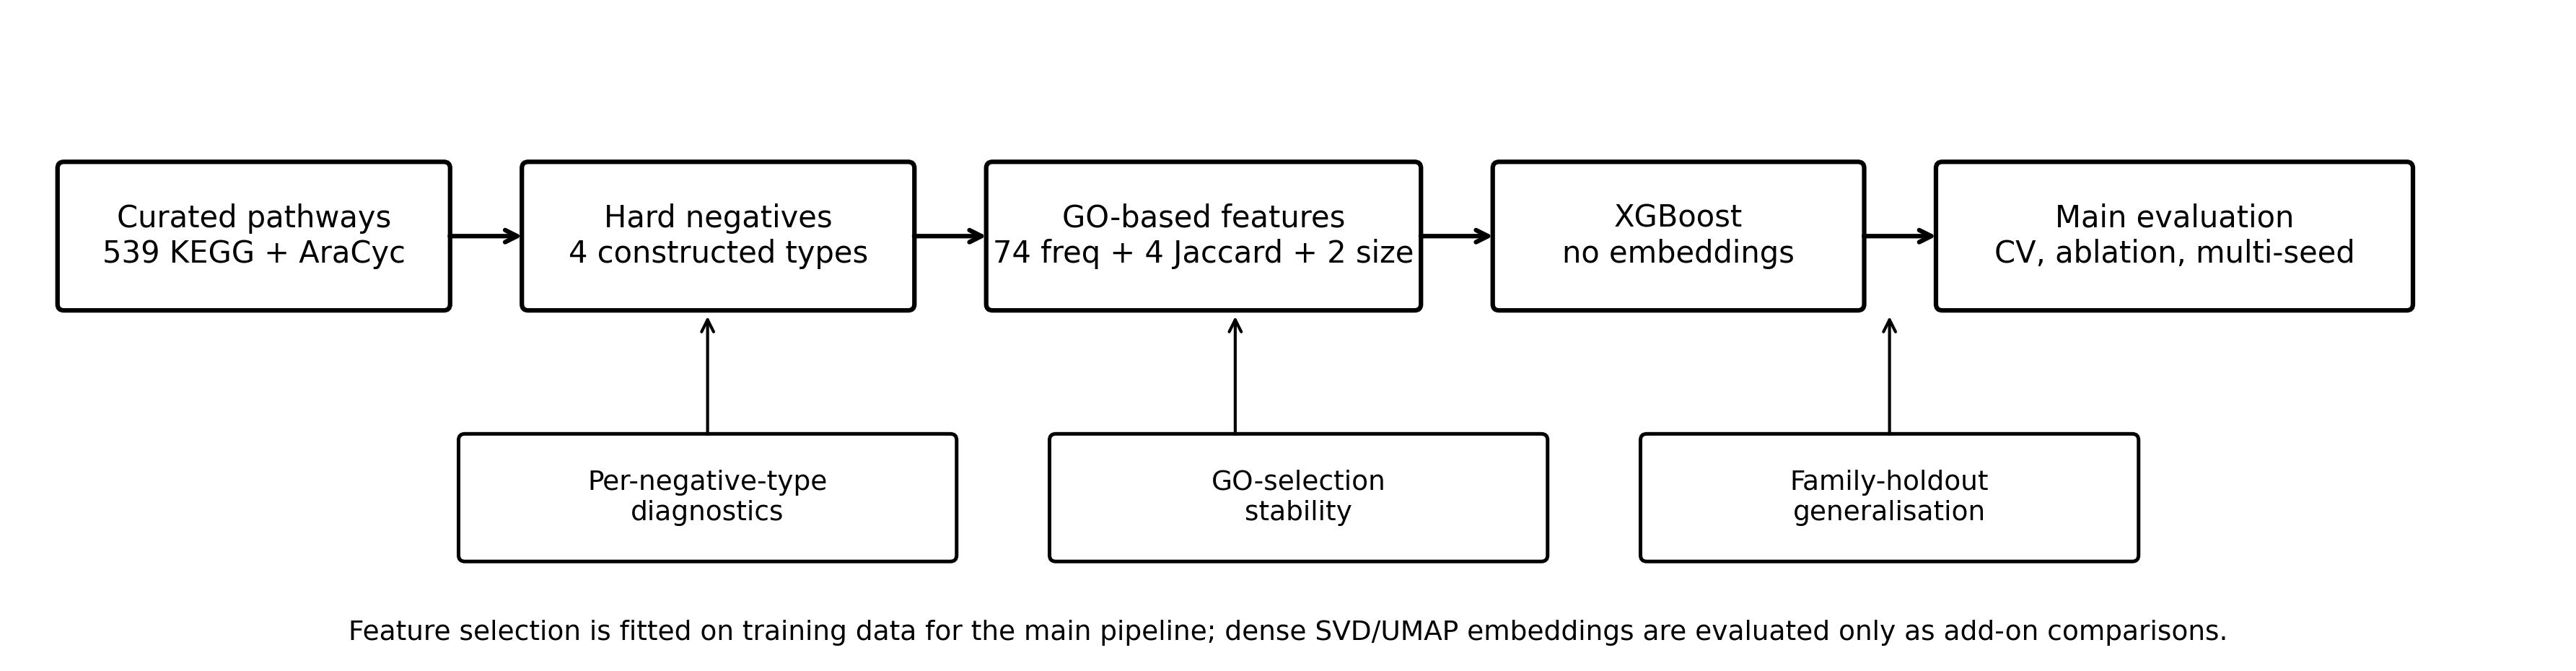
\includegraphics[width=0.92\textwidth]{figures/fig1_workflow_v6.png}
\caption{Overview of the final no-embedding PathwayML-Ath workflow: curated pathways, hard-negative generation, training-only GO selection, GO/Jaccard/size feature construction, XGBoost training, and evaluation through multi-seed, negative-type, and pathway-family validation.}
\label{fig:1}
\end{figure}
\subsection{Hard-negative design}
The negative class was designed to prevent trivial separation from curated pathways. Two negatives were generated per positive pathway, giving 1,078 negatives. Four negative types were used in roughly equal numbers.

Jaccard-matched random sets were sampled from the background gene pool and retained only when their internal Jaccard mean exceeded the 25th percentile of real pathways. Co-annotation clusters began with a seed gene, expanded with GO-similar neighbours, and then added random noise so that the set retained partial coherence without being a known pathway. Cross-pathway chimeras merged genes from two or three unrelated pathways. Shuffled pathways replaced 40-60\% of genes in a real pathway with background genes. Together, these controls force the model to learn more than set size or a single average-coherence threshold.

\subsection{Model training and evaluation}
The primary classifier was XGBoost with 500 trees, maximum depth 5, learning rate 0.03, and positive-class weighting for the 1:2 positive-to-negative ratio (Chen and Guestrin 2016). Random Forest and Logistic Regression were retained as reference baselines (Breiman 2001; Pedregosa et al. 2011). The 1,617 samples were split into training and held-out test sets using stratified random sampling, and all feature selection was restricted to the training split.

The seed-42 reference run used repeated stratified five-fold cross-validation with five repeats, giving 25 folds. Test metrics were computed once on the held-out test split. To assess stochastic stability, the entire pipeline was repeated for seeds 1-20. Each run regenerated negatives, train-test splits, GO-term selection, and model states.

\subsection{Additional validation analyses}
Per-negative-type evaluation was performed on the seed-42 held-out test set by separating the four negative types. This analysis reports which negative construction is hardest for the trained model.

Leave-one-family-out (LOFO) validation grouped curated pathways into ten broad families based on KEGG categories and AraCyc pathway naming. In each fold, one pathway family was withheld, new negatives were generated for that fold, GO selection was recomputed on training families only, and the model was evaluated on the held-out family. This design is stricter than a random split because the classifier cannot see any pathway from the held-out family during training.

Candidate scoring was used as a diagnostic validation rather than as a discovery claim. Four deterministic gene sets were scored across all seed-specific models: C2, a photosynthesis positive control; C3, a ubiquitin-mediated proteolysis positive control; C4, a deliberately mixed starch/random negative control; and C1, a stress/glutathione boundary example spanning CYP450 and GST-related genes. Hypergeometric ORA with Bonferroni correction was applied to each candidate against the curated pathway catalogue.

\section{Results}
\subsection{Reference classifier performance}
The seed-42 reference model produced an 80-dimensional feature vector and strong held-out performance. XGBoost achieved repeated-CV AUROC of 0.952 $\pm$ 0.002 SE, held-out AUROC of 0.948, AUPRC of 0.892, and F1 of 0.831 (Table 3). Random Forest was close behind, while Logistic Regression remained competitive but lower, indicating that much of the signal is captured by the engineered feature space and that tree-based interactions add a modest performance gain.

\begin{table}[H]
\centering
\caption{Seed-42 reference-run model performance. CV AUROC is mean $\pm$ SE over 25 repeated-CV folds.}
\label{tab:3}
\scriptsize
\resizebox{\textwidth}{!}{%
\begin{tabular}{lcccc}
\toprule
Model & CV AUROC & Test AUROC & Test AUPRC & Test F1 \\
\midrule
XGBoost & 0.952 $\pm$ 0.002 SE & 0.948 & 0.892 & 0.831 \\
Random Forest & 0.946 $\pm$ 0.002 SE & 0.94 & 0.879 & 0.821 \\
Logistic Regression & 0.911 $\pm$ 0.003 SE & 0.924 & 0.86 & 0.802 \\
\bottomrule
\end{tabular}%
}
\end{table}

\begin{figure}[H]
\centering
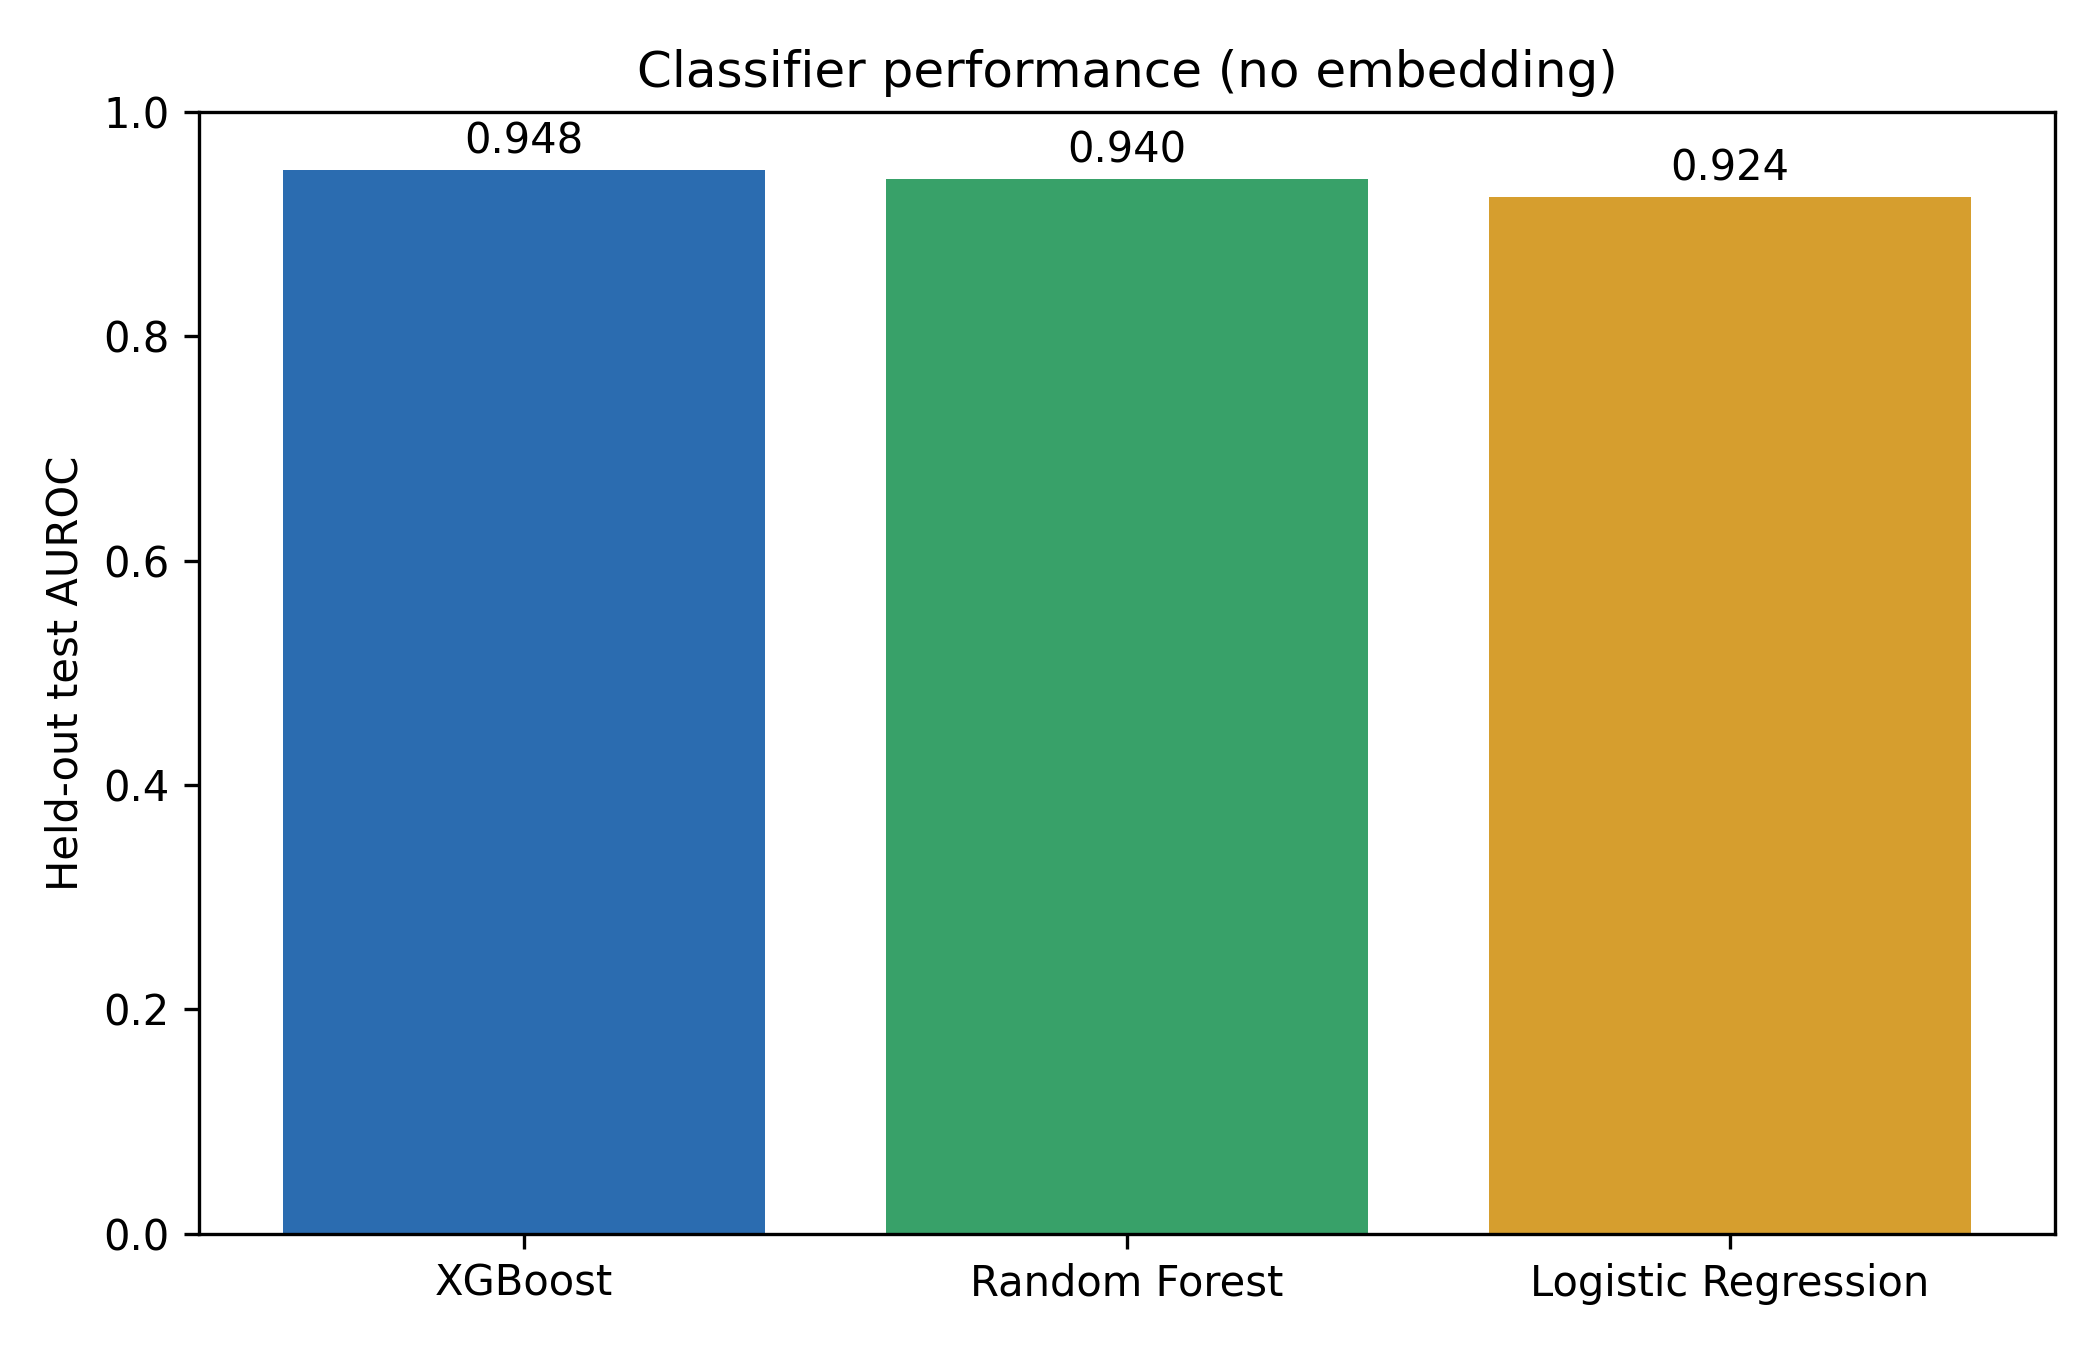
\includegraphics[width=0.92\textwidth]{figures/fig2_classifier_performance.png}
\caption{Held-out AUROC for the seed-42 no-embedding model comparison.}
\label{fig:2}
\end{figure}
\subsection{Multi-seed reproducibility}
Across 20 complete pipeline reruns, XGBoost remained stable. Mean test AUROC was 0.955 $\pm$ 0.010 SD and mean AUPRC was 0.909 $\pm$ 0.024 SD (Table 4). The full-pipeline design is important: these runs did not merely retrain the same matrix, but regenerated negatives, splits, selected GO terms, and model states.

GO-term selection varied more than model performance. The selected GO feature count ranged from 54 to 157, but the Pearson correlation between selected GO count and test AUROC was only r = -0.036. This supports the interpretation that there is a stable functional signal distributed across a recurrent pool of GO terms, rather than a single fragile selected-term list.

\begin{table}[H]
\centering
\caption{XGBoost stability across 20 independent full-pipeline runs.}
\label{tab:4}
\scriptsize
\resizebox{\textwidth}{!}{%
\begin{tabular}{lccccc}
\toprule
Metric & Mean & SD & SE & Min & Max \\
\midrule
Test AUROC & 0.955 & 0.010 & 0.002 & 0.933 & 0.972 \\
Test AUPRC & 0.909 & 0.024 & 0.005 & 0.847 & 0.940 \\
Test F1 & 0.839 & 0.023 & 0.005 & 0.793 & 0.892 \\
Selected GO terms & 106.6 & 39.0 & 8.7 & 54 & 157 \\
\bottomrule
\end{tabular}%
}
\end{table}

\begin{table}[H]
\centering
\caption{GO feature-selection stability across 20 seeds.}
\label{tab:5}
\scriptsize
\resizebox{\textwidth}{!}{%
\begin{tabular}{lc}
\toprule
Measure & Value \\
\midrule
Selected GO terms per seed & 54-157; mean 106.6, SD 39.0 \\
Unique GO terms selected at least once & 184 \\
Core terms selected in >=75\% of seeds & 57 \\
Recurrent terms selected in >=50\% of seeds & 127 \\
Mean pairwise Jaccard among selected-term sets & 0.524 $\pm$ 0.143 \\
Correlation between selected GO count and test AUROC & r = -0.036 \\
\bottomrule
\end{tabular}%
}
\end{table}

\begin{figure}[H]
\centering
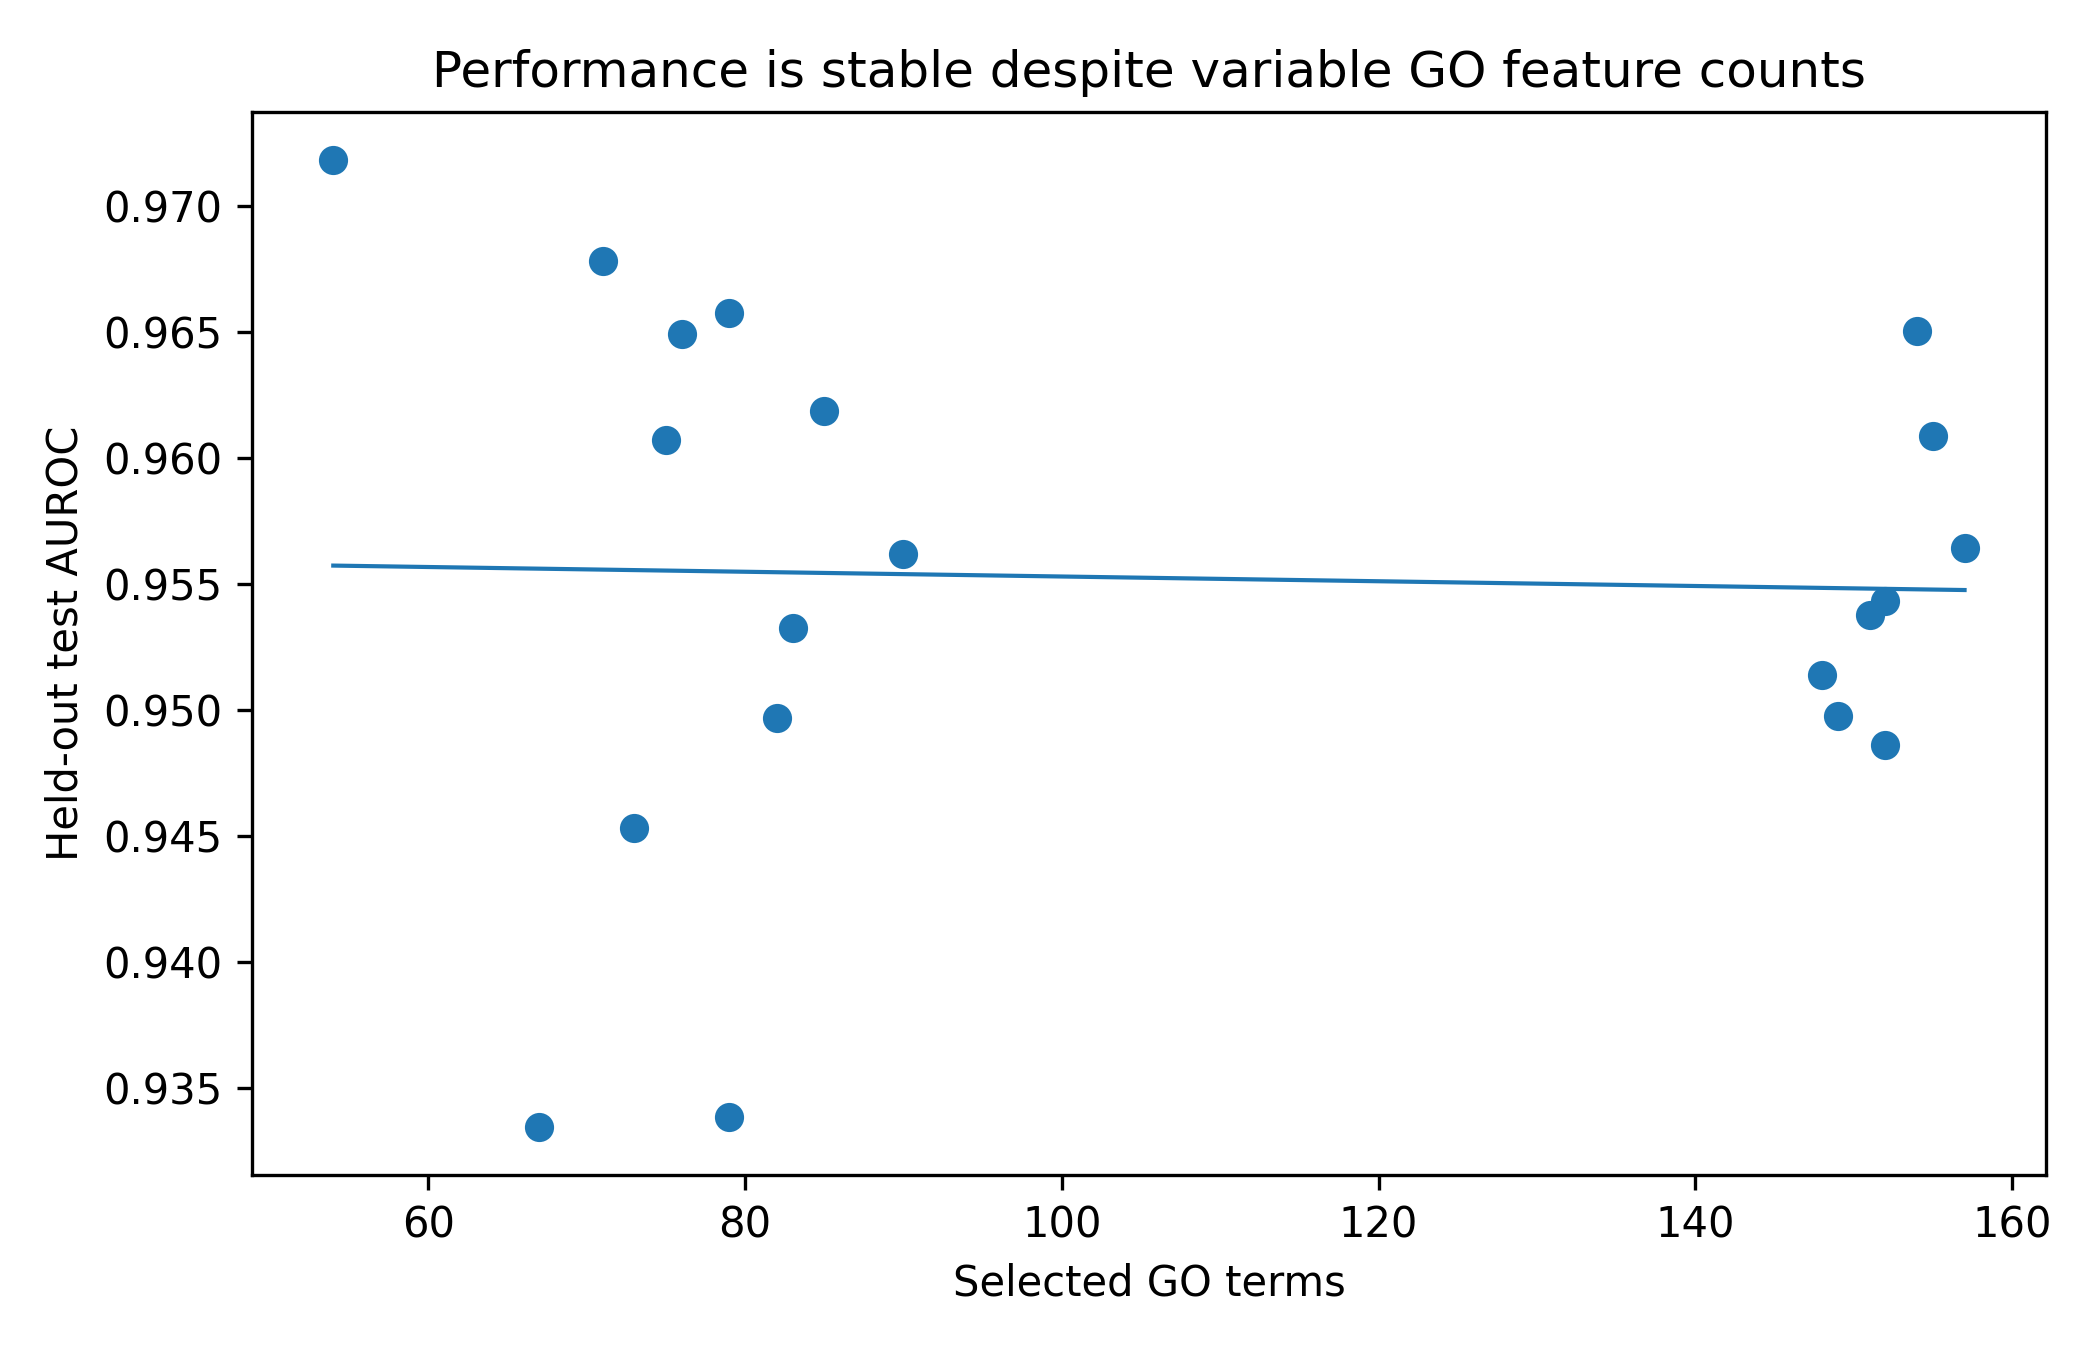
\includegraphics[width=0.92\textwidth]{figures/fig10_performance_vs_go_count.png}
\caption{Performance is stable despite variation in selected GO feature count. The fitted line is nearly flat, consistent with the weak correlation between GO count and test AUROC.}
\label{fig:3}
\end{figure}
\begin{figure}[H]
\centering
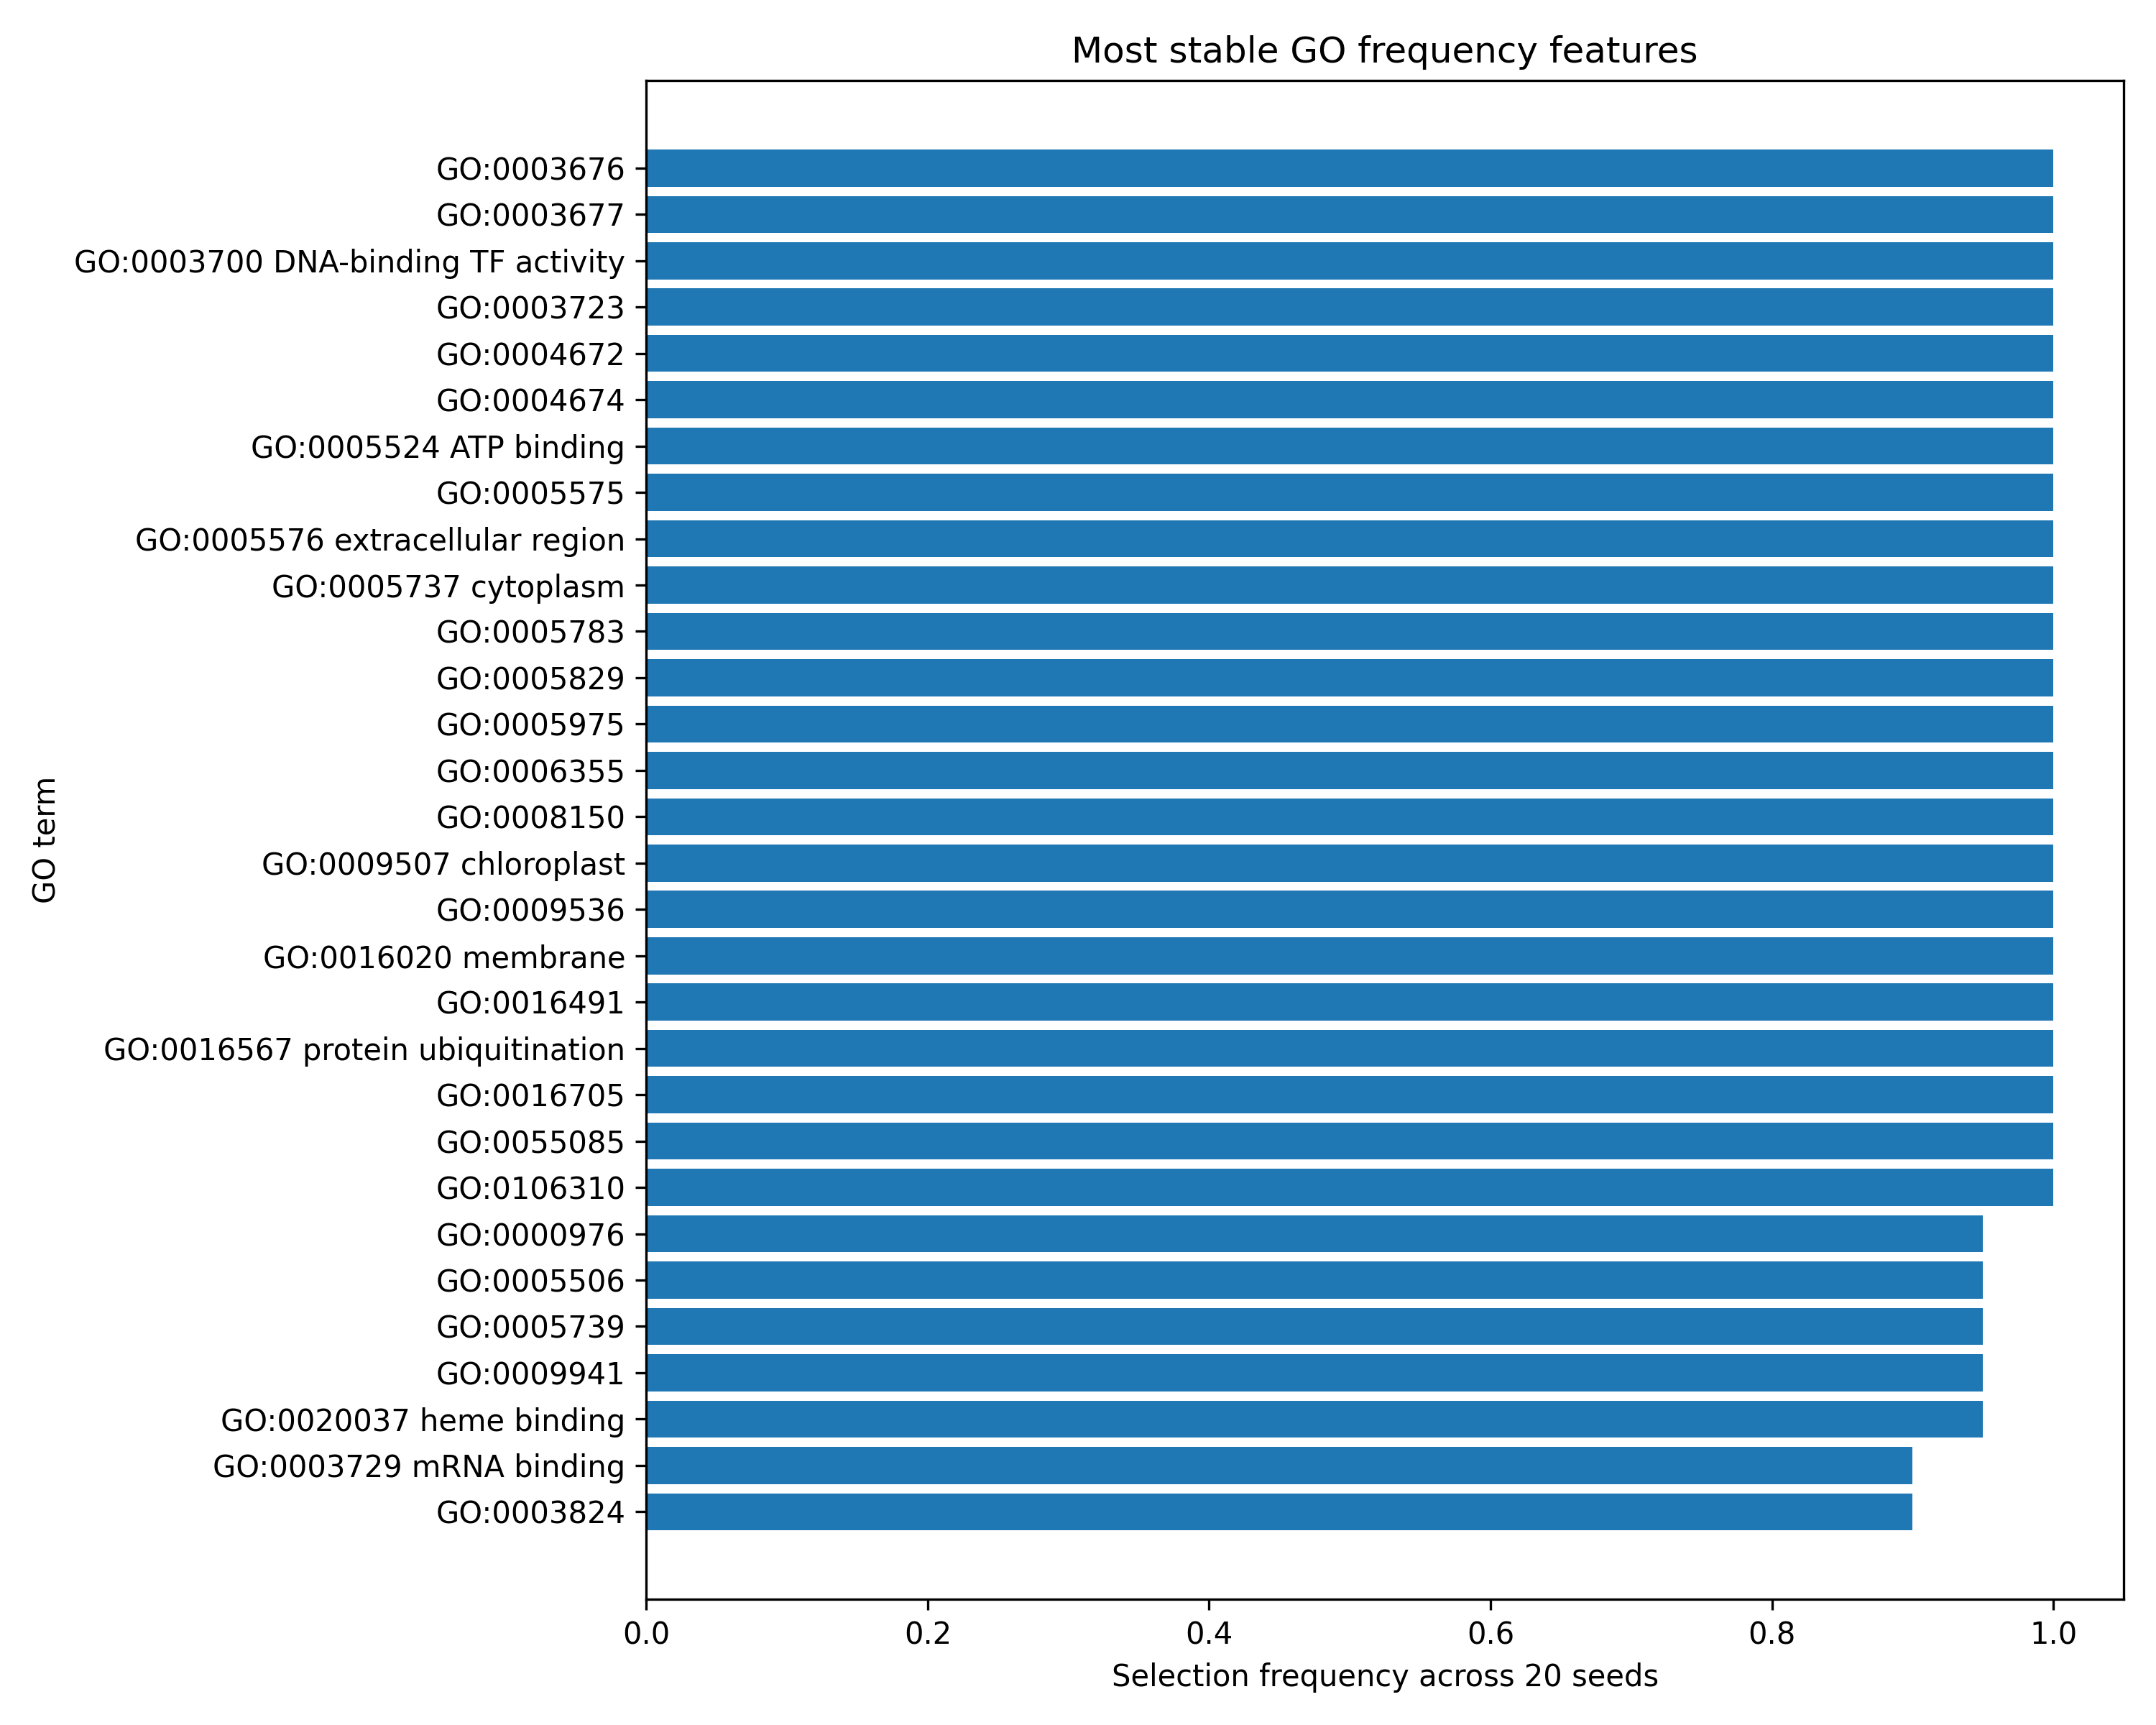
\includegraphics[width=0.92\textwidth]{figures/fig8_go_selection_stability.png}
\caption{Most frequently selected GO terms across 20 seeds. The stable core terms recur even though the total selected feature count varies.}
\label{fig:4}
\end{figure}
\subsection{Feature ablation}
Ablation confirms that the final model depends on both GO-frequency content and pairwise Jaccard coherence. Removing GO frequencies reduced test AUROC from 0.948 to 0.838, the largest single loss. Removing Jaccard statistics reduced test AUROC to 0.927, while removing size features reduced it only to 0.940 (Table 6). GO frequencies alone achieved AUROC 0.907, showing that functional-content information is strong. Jaccard alone achieved AUROC 0.800, showing that pairwise coherence is informative even without GO-term identity.

The cumulative addition experiment is more revealing than single removal. Size alone was not useful (AUROC 0.468). Adding Jaccard increased AUROC to 0.841, and adding GO frequencies completed the model at 0.948. Thus, Jaccard features provide the first large gain from a minimal baseline, while GO frequencies provide the larger absolute contribution to the final model.

\begin{table}[H]
\centering
\caption{Feature ablation and cumulative addition in the seed-42 run.}
\label{tab:6}
\scriptsize
\resizebox{\textwidth}{!}{%
\begin{tabular}{lccccc}
\toprule
Configuration & d & CV AUROC & Test AUROC & Test AUPRC & Delta vs full \\
\midrule
Full model & 80 & 0.952 $\pm$ 0.002 & 0.948 & 0.892 & +0.000 \\
-GO freq & 6 & 0.827 $\pm$ 0.006 & 0.838 & 0.769 & -0.110 \\
-Jaccard & 76 & 0.931 $\pm$ 0.002 & 0.927 & 0.853 & -0.021 \\
-Size & 78 & 0.945 $\pm$ 0.002 & 0.94 & 0.881 & -0.008 \\
GO freq only & 74 & 0.921 $\pm$ 0.002 & 0.907 & 0.825 & -0.041 \\
Jaccard only & 4 & 0.791 $\pm$ 0.007 & 0.8 & 0.714 & -0.148 \\
Size only & 2 & 0.512 $\pm$ 0.007 & 0.468 & 0.303 & -0.480 \\
Cumul: Size & 2 & 0.512 $\pm$ 0.007 & 0.468 & 0.303 & -0.480 \\
Cumul: +Jaccard & 6 & 0.826 $\pm$ 0.006 & 0.841 & 0.768 & -0.107 \\
Cumul: +GO freq & 80 & 0.952 $\pm$ 0.002 & 0.948 & 0.892 & +0.000 \\
\bottomrule
\end{tabular}%
}
\end{table}

\noindent\textit{Delta vs full is computed from the full-model seed-42 test AUROC of 0.948.}

\begin{figure}[H]
\centering
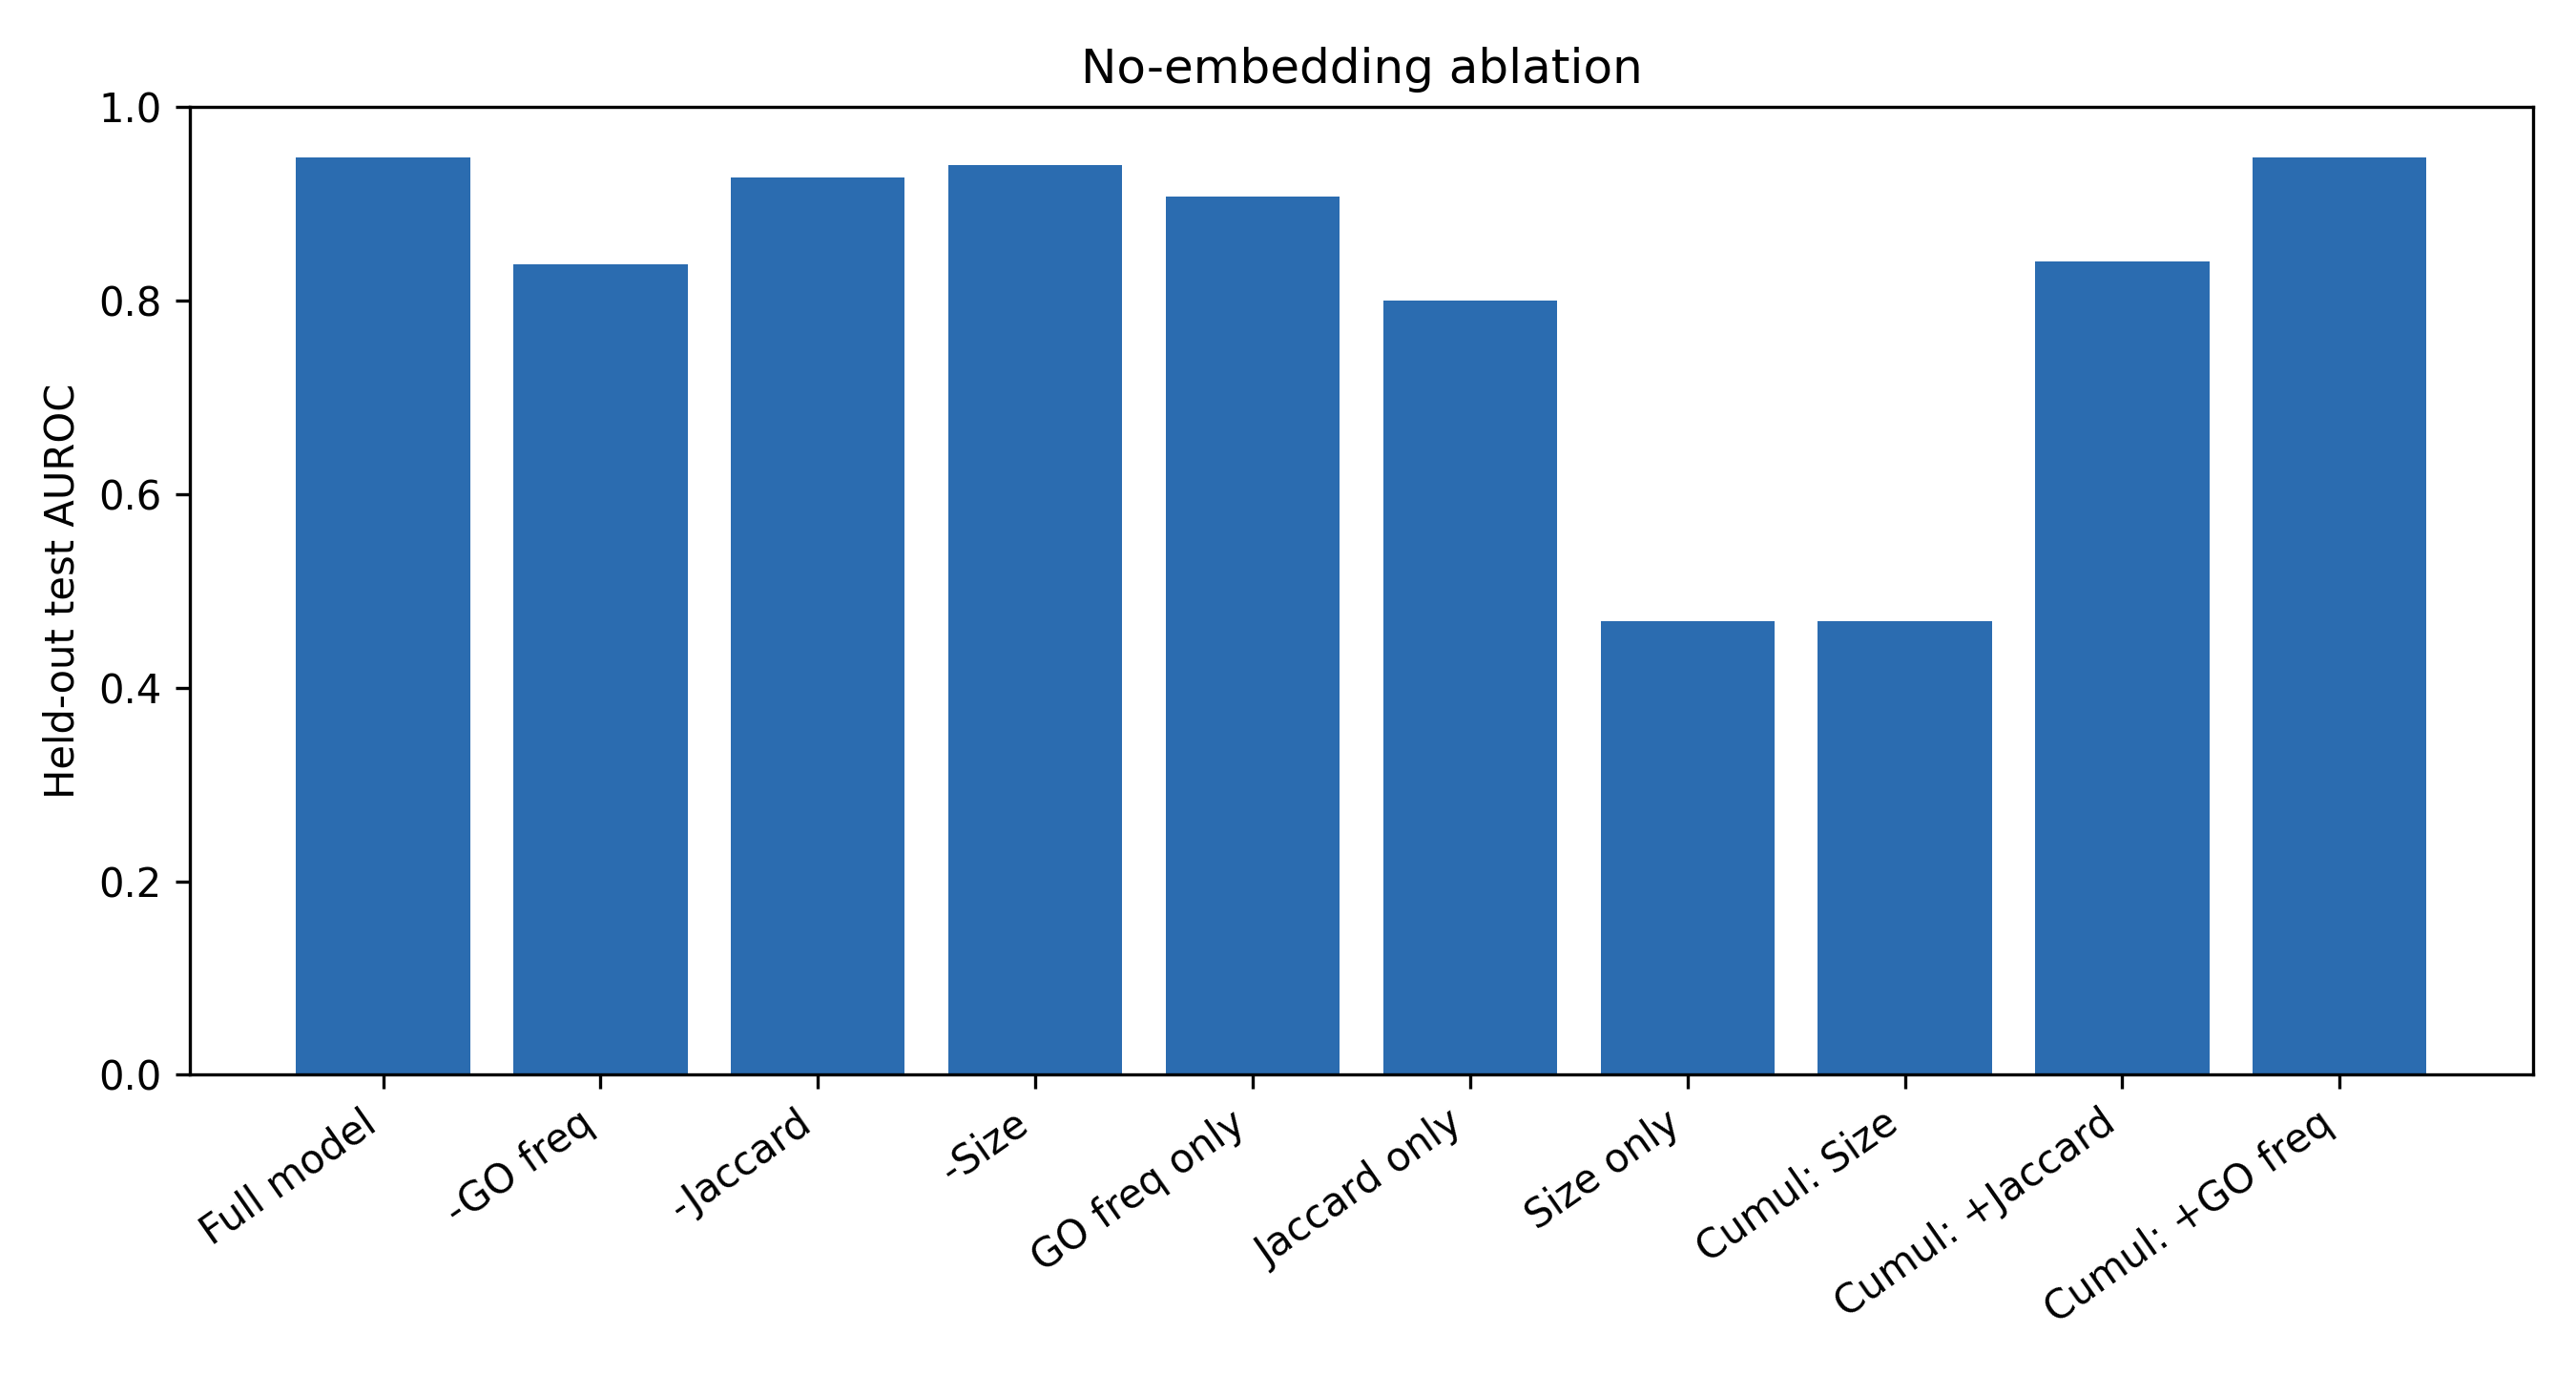
\includegraphics[width=0.92\textwidth]{figures/fig6_ablation.png}
\caption{No-embedding ablation results. The largest loss occurs when GO-frequency features are removed; Jaccard features are also necessary for strong performance.}
\label{fig:5}
\end{figure}
\subsection{Per-negative-type difficulty}
The mixed negative benchmark is not uniformly difficult. When the held-out negatives were separated by construction type, cross-pathway chimeras were the hardest controls (AUROC 0.876, AUPRC 0.911), whereas Jaccard-matched random sets and co-annotation clusters were easier (Table 7). This result corrects the earlier assumption that co-annotation clusters would necessarily be the hardest type. Chimeras are challenging because they contain fragments of real pathways and therefore can preserve local functional coherence while disrupting single-pathway consistency.

This analysis also clarifies how to interpret the headline AUROC of 0.948. It is performance against a mixed benchmark containing easy and hard negatives, not a claim that every biologically plausible non-pathway module can be rejected with equal confidence.

\begin{table}[H]
\centering
\caption{Seed-42 performance by negative type on the held-out test set.}
\label{tab:7}
\scriptsize
\resizebox{\textwidth}{!}{%
\begin{tabular}{lcccccc}
\toprule
Comparison & n+ & n- & Test AUROC & Test AUPRC & Negative median score & Negative score IQR \\
\midrule
All mixed negatives & 108 & 216 & 0.948 & 0.892 & 0.023 & 0.004-0.179 \\
jaccard matched & 108 & 48 & 0.997 & 0.999 & 0.002 & 0.001-0.010 \\
co annotation & 108 & 48 & 0.979 & 0.99 & 0.006 & 0.002-0.041 \\
chimera & 108 & 66 & 0.876 & 0.911 & 0.217 & 0.071-0.565 \\
shuffled & 108 & 54 & 0.965 & 0.982 & 0.024 & 0.007-0.137 \\
\bottomrule
\end{tabular}%
}
\end{table}

\begin{figure}[H]
\centering
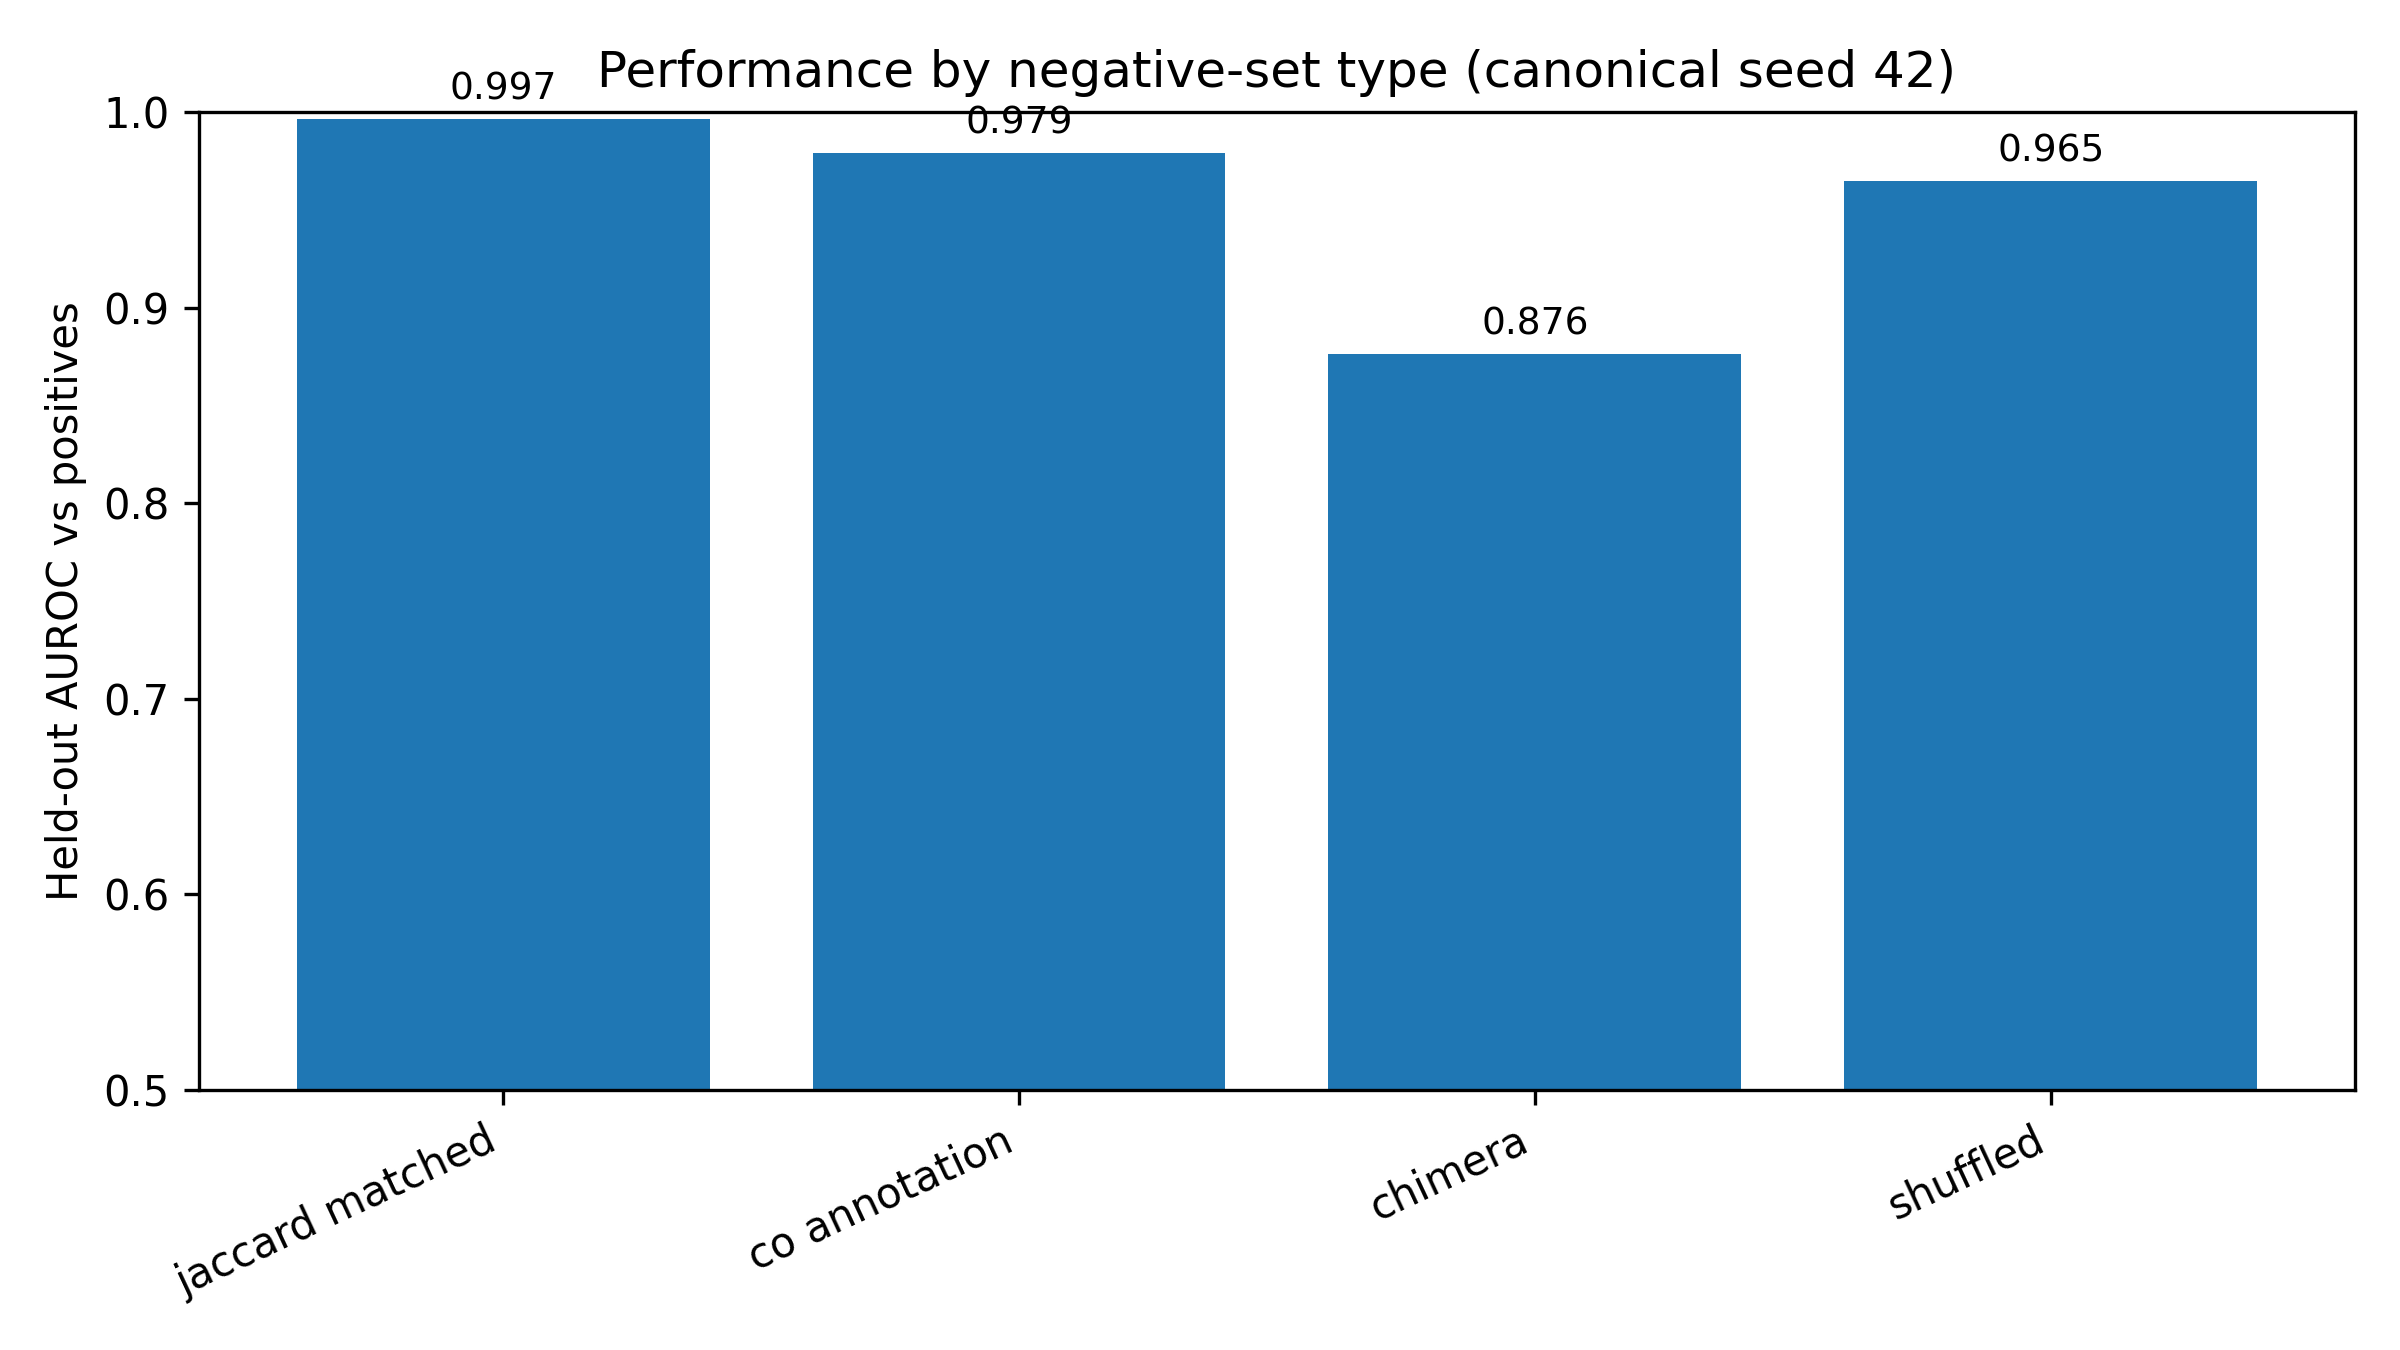
\includegraphics[width=0.92\textwidth]{figures/fig11_negative_type_performance.png}
\caption{Held-out AUROC by negative type. Cross-pathway chimeras are the most difficult controls in the recomputed analysis.}
\label{fig:6}
\end{figure}
\subsection{Leave-one-family-out generalisation}
LOFO validation tests whether the classifier generalises across broad pathway families rather than relying on family-specific GO signatures. Recomputed LOFO AUROC ranged from 0.861 to 0.957, and AUPRC ranged from 0.728 to 0.935 (Table 8). The lowest AUROC occurred for signalling/regulatory pathways, while carbohydrate and cofactor/vitamin metabolism achieved the highest AUROC values.

The LOFO results are more conservative and more useful than a random split. They show that the model retains above-chance discrimination when entire biological families are withheld. At the same time, family-to-family variation indicates that PathwayML-Ath should be reported with uncertainty estimates and not treated as a universal pathway detector.

\begin{table}[H]
\centering
\caption{Recomputed leave-one-family-out generalisation results.}
\label{tab:8}
\scriptsize
\resizebox{\textwidth}{!}{%
\begin{tabular}{lcccccc}
\toprule
Family & n pathways & Median size & Median Jaccard & GO terms & AUROC & AUPRC \\
\midrule
Cofactor/vitamin metabolism & 29 & 15 & 0.138 & 41 & 0.957 & 0.893 \\
Carbohydrate metabolism & 31 & 30 & 0.142 & 37 & 0.957 & 0.913 \\
Other AraCyc & 47 & 12 & 0.217 & 40 & 0.956 & 0.935 \\
Amino acid metabolism & 60 & 18 & 0.175 & 37 & 0.944 & 0.899 \\
Specialized/other biosynthesis & 160 & 12 & 0.217 & 40 & 0.937 & 0.867 \\
Lipid metabolism & 50 & 14 & 0.174 & 35 & 0.931 & 0.85 \\
Energy metabolism & 15 & 39 & 0.139 & 36 & 0.927 & 0.893 \\
Degradation/catabolism & 76 & 11 & 0.166 & 41 & 0.903 & 0.818 \\
Other KEGG/cellular & 58 & 62 & 0.132 & 40 & 0.894 & 0.773 \\
Signalling/regulatory & 13 & 27 & 0.147 & 37 & 0.861 & 0.728 \\
\bottomrule
\end{tabular}%
}
\end{table}

\begin{figure}[H]
\centering
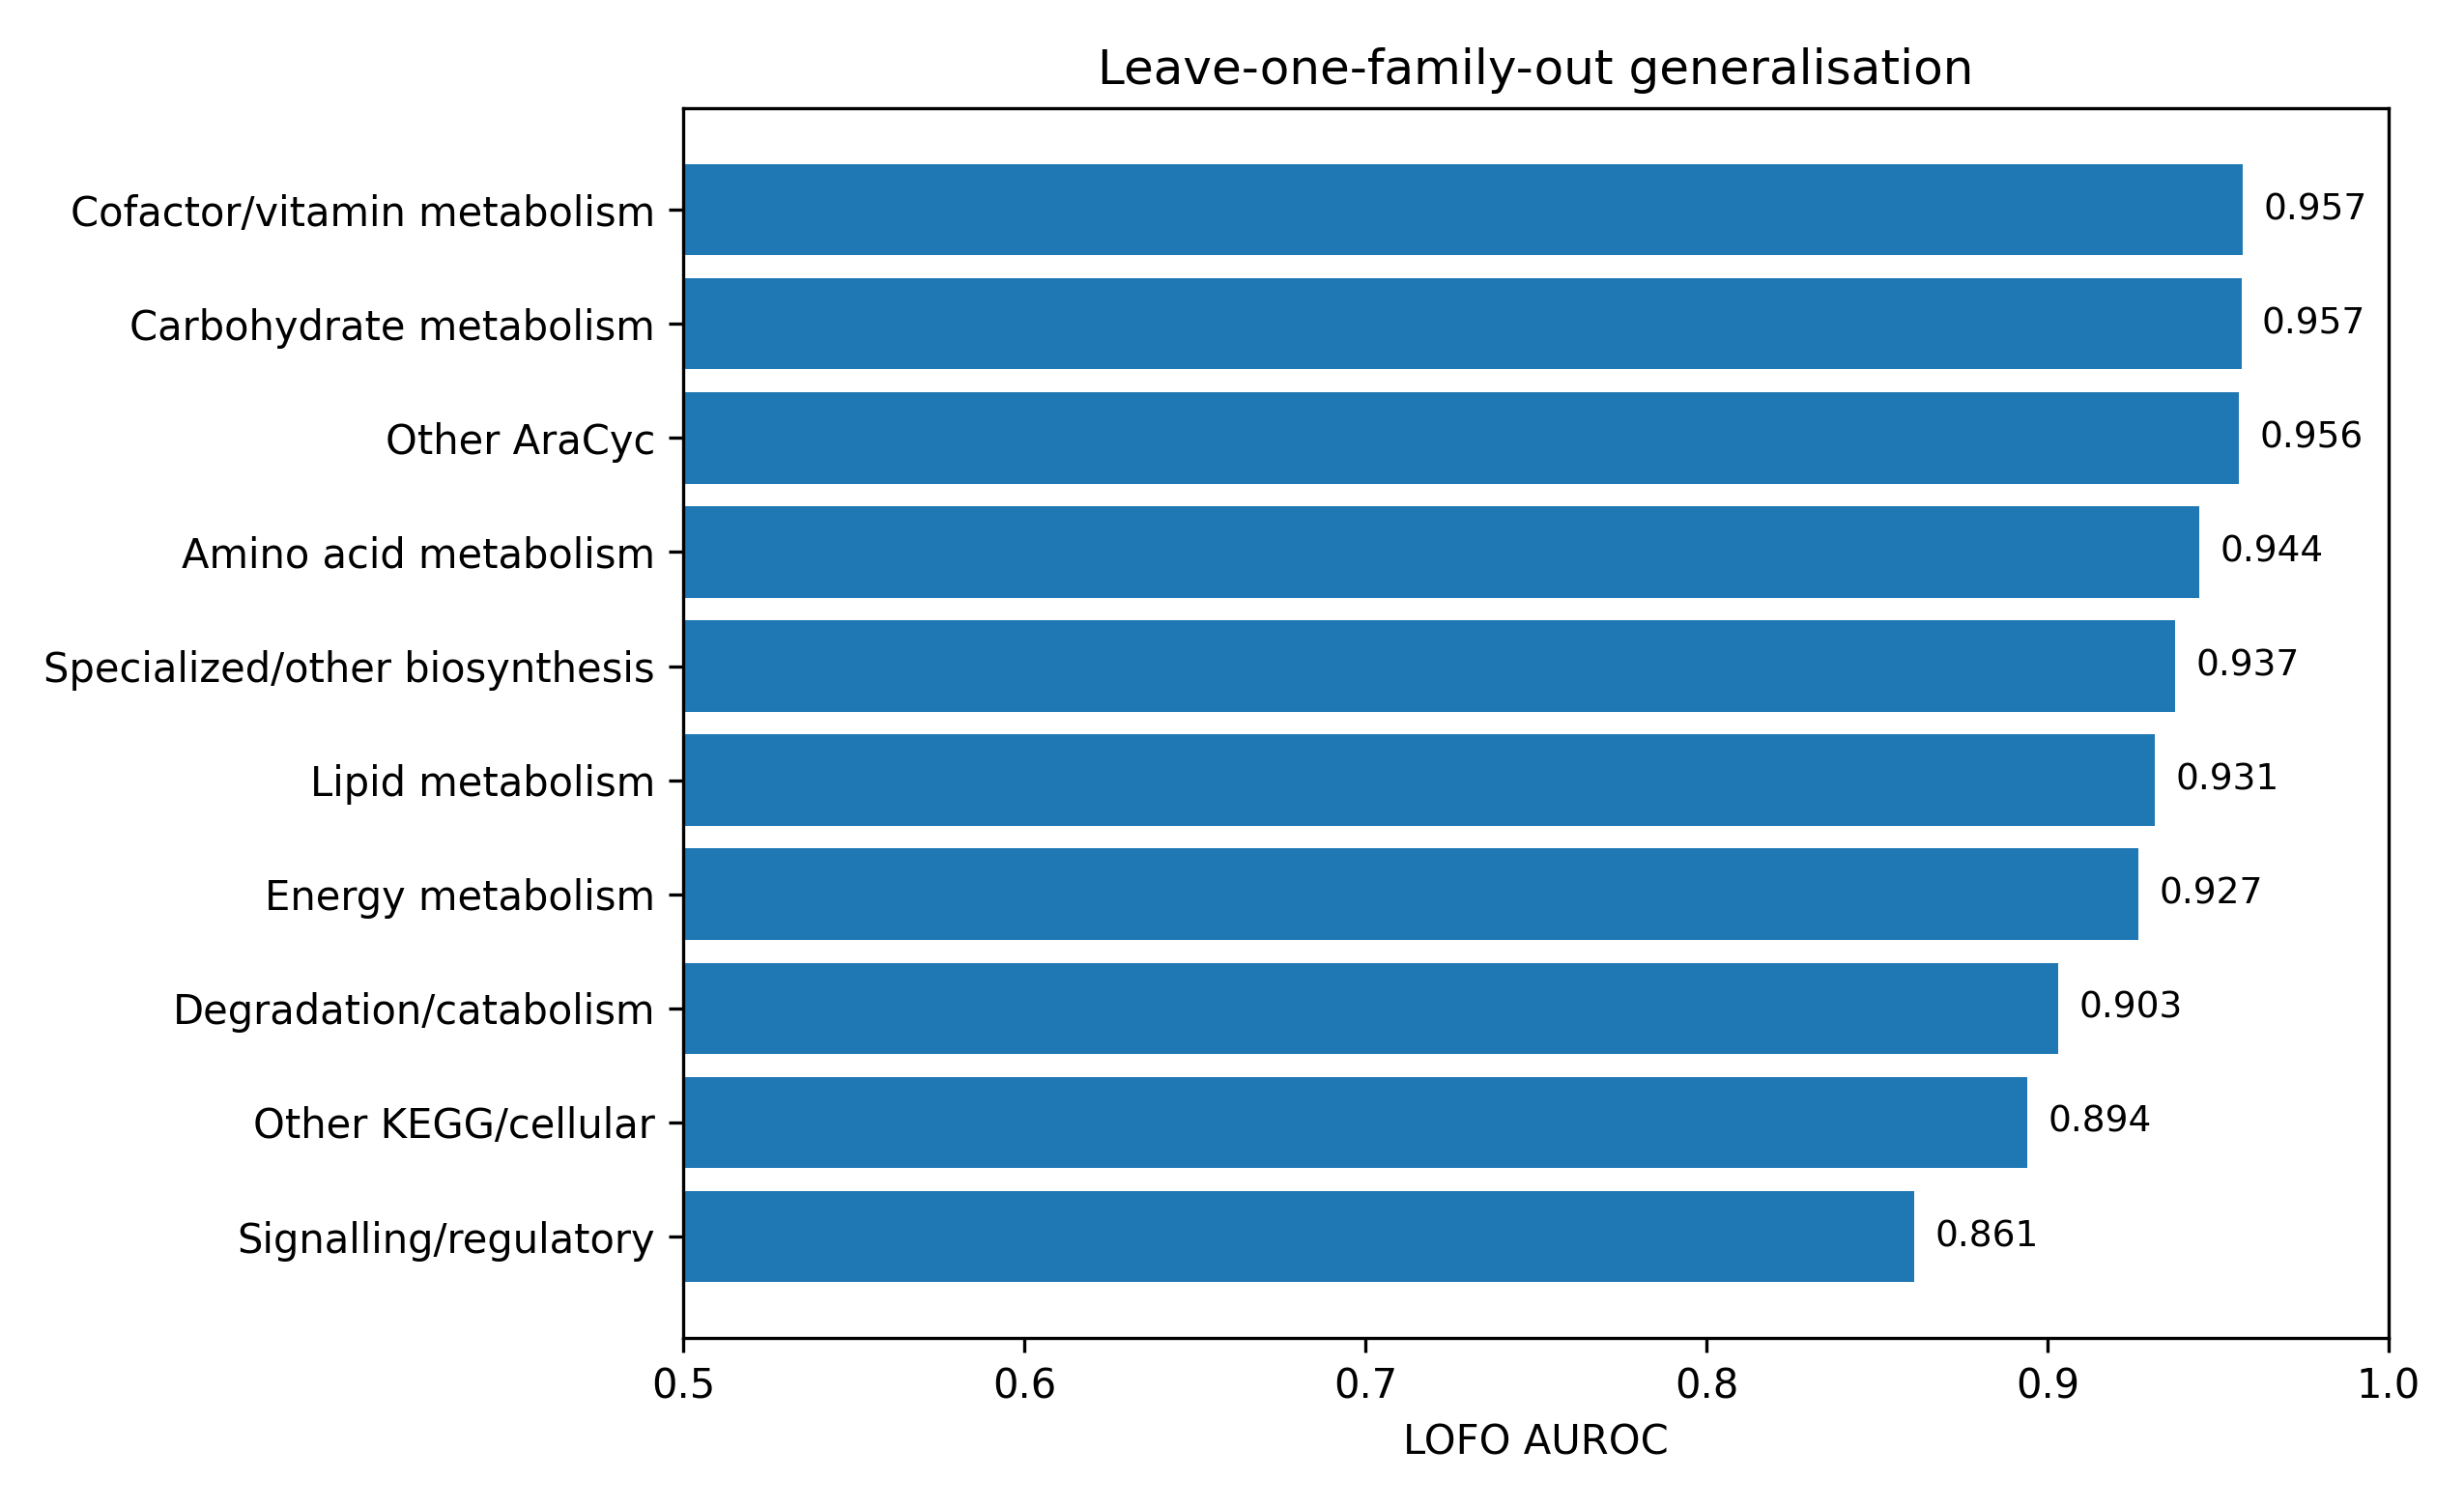
\includegraphics[width=0.92\textwidth]{figures/fig12_lofo_generalization.png}
\caption{Recomputed LOFO AUROC by pathway family. All families remain above chance, with the strongest family shift observed for signalling/regulatory pathways.}
\label{fig:7}
\end{figure}
\begin{figure}[H]
\centering
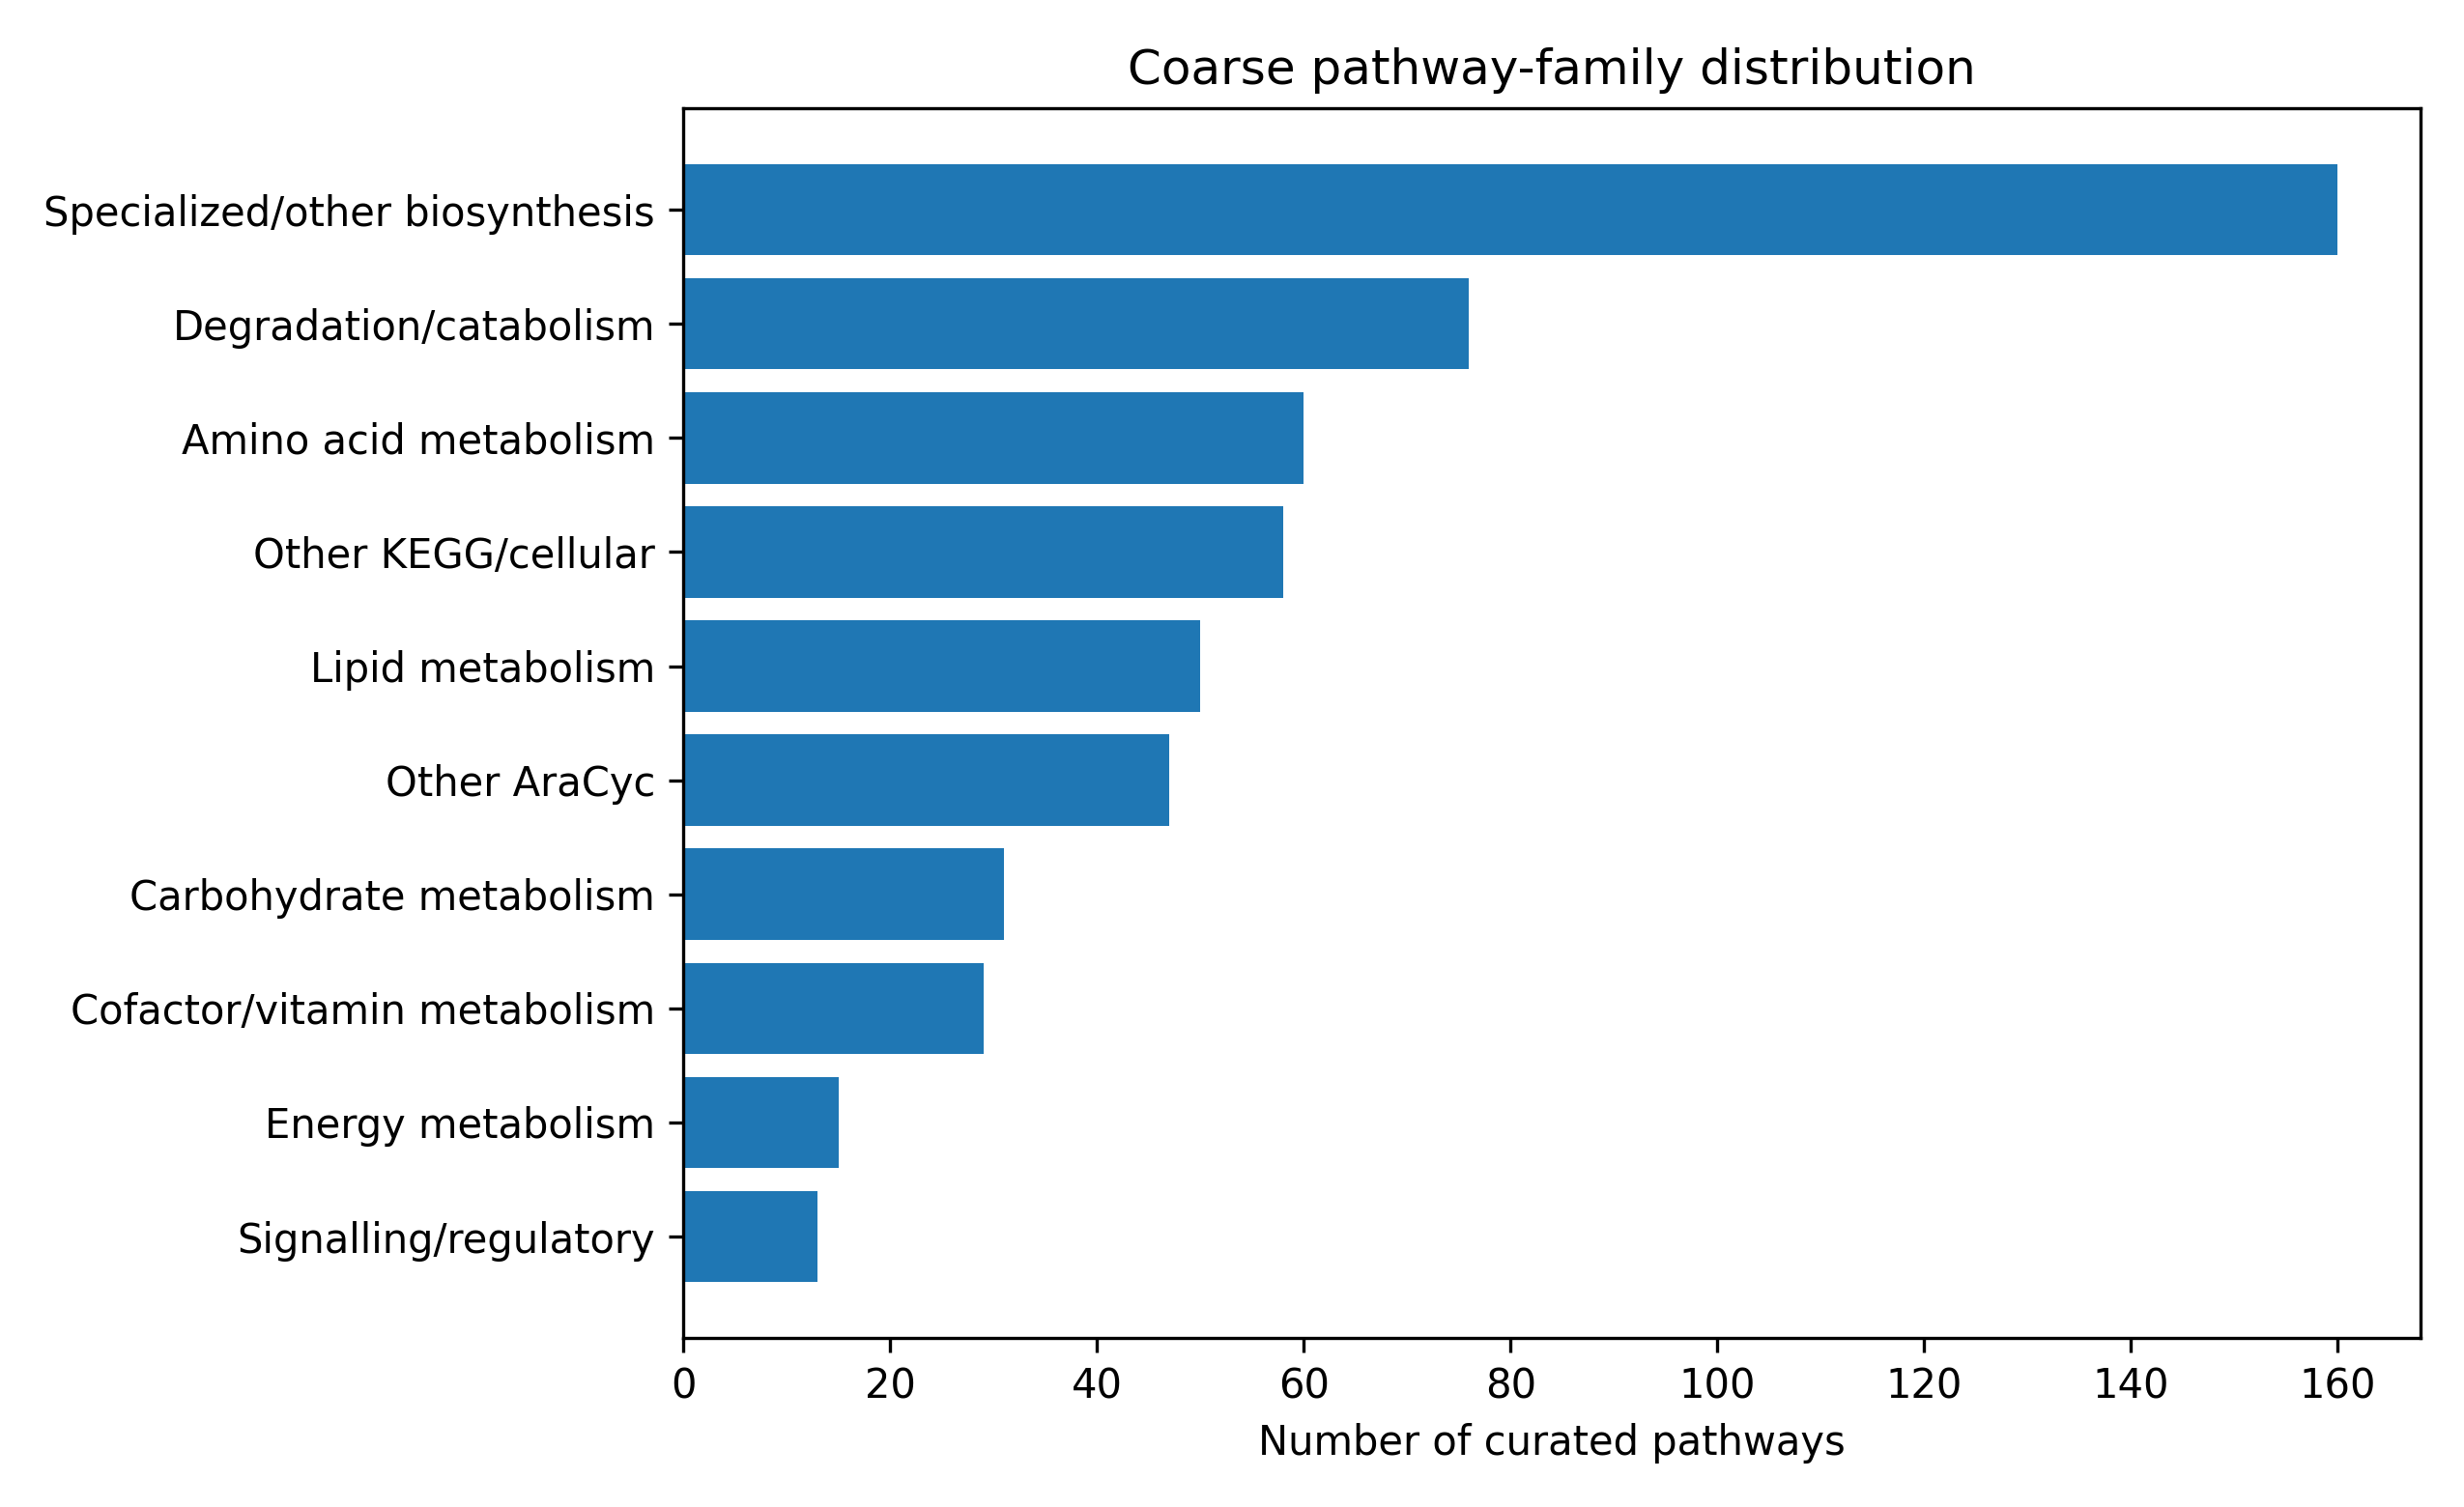
\includegraphics[width=0.92\textwidth]{figures/fig13_family_distribution.png}
\caption{Coarse family distribution among curated pathways used for LOFO validation.}
\label{fig:8}
\end{figure}
\subsection{Model interpretation}
SHAP attribution indicates that the highest-ranked feature is jaccard\_mean, followed by GO:0008150, pathway\_size, transcription-factor/DNA-binding features, and other Jaccard statistics (Table 9; Figure 9). The prominence of jaccard\_mean supports the coherence premise. Some generic GO features also appear among the top predictors; these should be interpreted partly as annotation-coverage and functional-composition signals rather than as specific mechanistic claims.

The important point is not that a single GO term explains pathway membership, but that the combination of functional content, pairwise sharing, and size-normalised structure produces a stable decision rule.

\begin{table}[H]
\centering
\caption{Top 12 seed-42 SHAP features for the XGBoost model.}
\label{tab:9}
\scriptsize
\resizebox{\textwidth}{!}{%
\begin{tabular}{lccc}
\toprule
Feature & Name / statistic & Mean |SHAP| & \% total \\
\midrule
jaccard\_mean & Mean pairwise GO Jaccard & 1.155 & 13.8 \\
GO:0008150 & biological process & 0.914 & 11.0 \\
pathway\_size & Gene-set size & 0.619 & 7.4 \\
GO:0003700 & DNA-binding transcription factor activity & 0.381 & 4.6 \\
GO:0003677 & DNA binding & 0.311 & 3.7 \\
jaccard\_std & SD of pairwise GO Jaccard & 0.266 & 3.2 \\
jaccard\_max & Maximum pairwise GO Jaccard & 0.231 & 2.8 \\
GO:0016020 & membrane & 0.220 & 2.6 \\
GO:0055085 & transmembrane transport & 0.202 & 2.4 \\
log\_size & log(1 + gene-set size) & 0.186 & 2.2 \\
GO:0005829 & cytosol & 0.177 & 2.1 \\
GO:0005515 & protein binding & 0.173 & 2.1 \\
\bottomrule
\end{tabular}%
}
\end{table}

\noindent\textit{Percent total is based on the summed mean absolute SHAP attribution across all features in the no-embedding model.}

\begin{figure}[H]
\centering

\includegraphics[width=0.92\textwidth]{figures/fig3_shap_analysis.png}
\caption{SHAP feature attribution for the no-embedding XGBoost model.}
\label{fig:9}
\end{figure}
\subsection{Candidate scoring and ORA comparison}
The candidate analysis was used as a diagnostic test of model behaviour. Known pathway subsets C2 and C3 scored highly, while the deliberately disrupted C4 set scored near zero across all seeds. C4 is particularly informative because ORA is significant against starch and sucrose metabolism, but the PathwayML-Ath score is near zero. This shows that the two methods answer different questions: ORA detects overlap with a known pathway, whereas PathwayML-Ath scores internal coherence of the submitted set.

C1 also receives a high score, but it is ORA-significant and overlaps glutathione metabolism. It is therefore not presented as a novel pathway. A cautious interpretation is that C1 is a stress/glutathione-associated boundary case consistent with known oxidative-stress biology, not a discovery result.

\begin{table}[H]
\centering
\caption{Candidate scoring and ORA comparison across seed-42 and 20-seed models.}
\label{tab:10}
\scriptsize
\resizebox{\textwidth}{!}{%
\begin{tabular}{lccccccc}
\toprule
Set & Role & n & Seed-42 score & 20-seed score & Closest overlap & ORA adj. p & Interpretation \\
\midrule
C1 & stress/glutathione boundary case & 17 & 0.883 & 0.877 $\pm$ 0.100 & Glutathione metabolism (0.412) & 1.19e-11 & not novel; ORA-supported boundary example \\
C2 & photosynthesis positive control & 11 & 0.924 & 0.823 $\pm$ 0.150 & Photosynthesis (1.000) & <1e-20 & known pathway positive control \\
C3 & ubiquitin proteolysis positive control & 14 & 0.895 & 0.958 $\pm$ 0.034 & Ubiquitin mediated proteolysis (1.000) & <1e-20 & known pathway positive control \\
C4 & mixed starch/random negative control & 9 & 0.001 & 0.002 $\pm$ 0.002 & Starch and sucrose metabolism (0.556) & 7.86e-07 & ORA-positive but ML-low disrupted set \\
\bottomrule
\end{tabular}%
}
\end{table}

\begin{figure}[H]
\centering
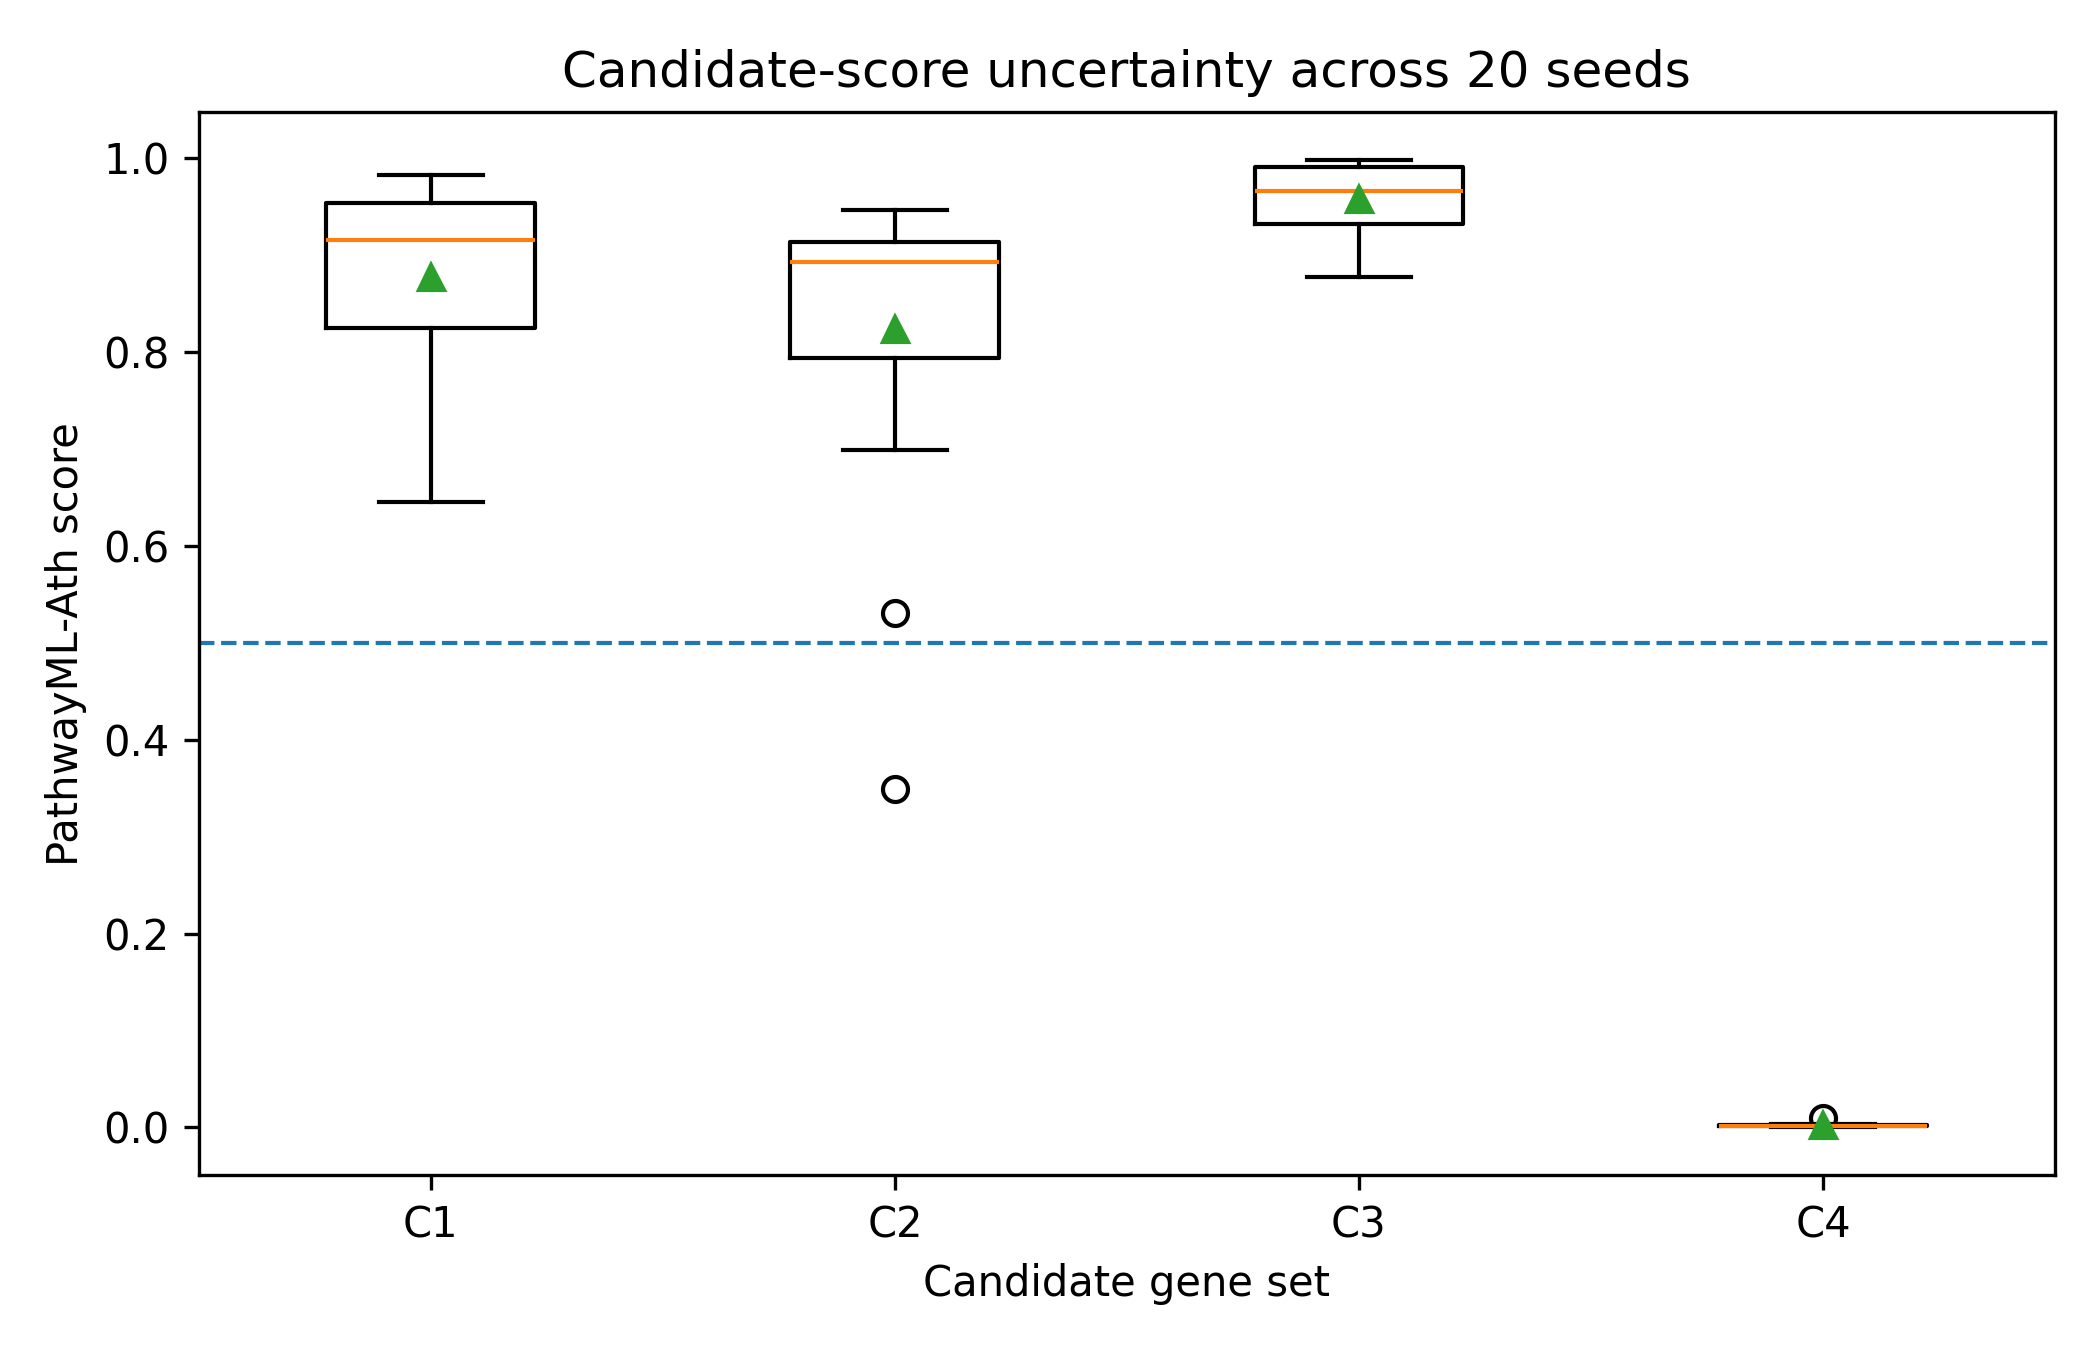
\includegraphics[width=0.92\textwidth]{figures/fig9_candidate_score_uncertainty.png}
\caption{Candidate-score uncertainty across 20 seed-specific models. C4 remains consistently low despite ORA significance.}
\label{fig:10}
\end{figure}
\begin{figure}[H]
\centering

\includegraphics[width=0.92\textwidth]{figures/fig4_candidates.png}
\caption{Seed-42 candidate score versus maximum curated-pathway Jaccard similarity.}
\label{fig:11}
\end{figure}
\section{Discussion}
\subsection{What PathwayML-Ath contributes}
PathwayML-Ath reframes pathway interpretation as a coherence-scoring problem. ORA and GSEA are valuable for testing known pathway catalogues, but they do not directly quantify whether an unranked gene set has pathway-like internal structure. This study shows that GO-frequency features and pairwise GO Jaccard statistics can learn that structure with strong held-out performance and reproducible multi-seed behaviour.

The strongest methodological contribution is not the use of XGBoost alone. It is the combination of interpretable GO-based features, hard-negative construction, training-only feature selection, full-pipeline multi-seed evaluation, per-negative-type analysis, and LOFO validation. These components make the result more defensible than a single random split.

\subsection{Feature interpretation}
The ablation results separate two related concepts. GO frequencies describe what functions are present. Pairwise Jaccard statistics describe how consistently those functions are shared across members. GO frequencies provide the largest individual signal in the final model, while Jaccard statistics supply the first large gain from a minimal baseline and remain the top SHAP feature. This supports a biological interpretation in which pathway-like gene sets require both specific functional content and internal pairwise coherence.

Size features play a smaller role. The size-only model is below chance, and removing size from the full model reduces AUROC by only 0.008. Size is therefore useful mainly for calibration, not for discrimination.

\subsection{Why the negative design matters}
Easy random negatives can inflate performance by allowing the classifier to separate curated pathways from incoherent gene lists. The recomputed negative-type analysis shows that cross-pathway chimeras are the hardest controls. This is plausible: chimeras combine genuine pathway fragments, preserving local GO structure while disrupting single-pathway consistency. A good future benchmark should increase the share and diversity of chimeric and co-annotation controls.

The mixed benchmark remains useful because experimental gene clusters vary in difficulty. Some will be random-like, some partially coherent, and some chimeric. Reporting both the mixed benchmark and per-type performance gives readers a clearer view of what the classifier can and cannot do.

\subsection{Stability and the GO-term count issue}
The number of selected GO terms changes across seeds because each seed changes negative generation, train-test splits, and mutual-information rankings. This variation should not be hidden. The key finding is that selected GO count is not meaningfully correlated with test AUROC, and many GO terms recur across seeds. In practice, the seed-42 model provides an inspectable reference, while the 20-seed distribution provides uncertainty estimates.

This treatment turns a potential reproducibility criticism into a documented property of the method. The classifier is not dependent on one exact GO list; it draws from a stable recurrent functional signal.

\subsection{Generalisation beyond random splits}
Random train-test splits are necessary but insufficient for a pathway classifier because related pathways may share GO signatures. LOFO validation provides a stricter assessment by withholding entire pathway families. The recomputed LOFO results remain above chance across all families but vary substantially by family. This finding is stronger and more honest than a single high random-split AUROC: PathwayML-Ath learns transferable signal, but transfer is not uniform across biology.

Signalling and regulatory pathways are the most difficult in the current LOFO analysis. This may reflect smaller sample counts, more diffuse annotations, or weaker metabolic-pathway structure compared with enzyme-dominated families. Further work should examine these sources separately.

\subsection{Relationship with ORA and candidate interpretation}
The candidate analysis clarifies the intended use of the tool. PathwayML-Ath is not a replacement for ORA. It is a complementary score: ORA reports overlap with existing curated pathways, while PathwayML-Ath reports model-estimated internal coherence. C4 demonstrates that overlap alone is not enough; the set overlaps starch and sucrose metabolism but is internally disrupted and receives a near-zero coherence score.

A high PathwayML-Ath score with no ORA signal would be the most interesting discovery scenario, but that scenario was not observed among the four diagnostic candidates. This is an important negative result. The model should be used to prioritise gene sets for further analysis, not to declare novel pathways without independent evidence.

\subsection{Limitations}
Several limitations remain. First, the model depends on the availability and quality of GO annotations. Genes with sparse or uninformative GO annotations contribute little to GO-frequency and Jaccard features. Second, the current model was trained only on Arabidopsis and should not be assumed to transfer to other species without retraining or external validation. Third, the negative classes are constructed controls rather than experimentally confirmed non-pathways. Fourth, the candidate gene sets are diagnostic examples and not experimental discoveries.

The final no-embedding model is intentionally conservative. It does not rule out embeddings in general. Co-expression-derived gene embeddings, protein language model representations, or graph-based features from metabolic or protein-interaction networks may add information not present in GO annotations. Those extensions should be evaluated against the same hard-negative, multi-seed, and LOFO framework before being adopted.

\section{Conclusion}
This study establishes PathwayML-Ath as an interpretable, reproducible classifier for GO-based pathway-level gene-set coherence in Arabidopsis thaliana. The recomputed no-embedding pipeline achieves strong random-split performance, remains stable over 20 full-pipeline seeds, and generalises above chance under leave-one-family-out testing.

The most defensible conclusion is deliberately narrow: GO-frequency and pairwise GO Jaccard features can distinguish curated Arabidopsis pathways from constructed hard negatives and can prioritise gene sets for further inspection. They do not, by themselves, prove that a high-scoring gene set is a novel pathway. Used alongside ORA, overlap checks, seed-level uncertainty, and biological validation, PathwayML-Ath provides a rigorous framework for ranking pathway-like gene sets.

\section{Data Availability and Reproducibility}
The source of truth for this revision is the local package PathwayML-Ath\_recomputed\_code\_data\_20260511\_170351.zip. The recomputed handoff states that the current data/ directory was treated as frozen input and that outputs in tables/ and figures/ were regenerated from code. The LaTeX draft in that package is explicitly not a source of truth.

The core commands recorded in the package were: python -m py\_compile *.py; python run\_no\_embedding\_reproducible.py --seed 42 --no-figures; python run\_no\_embedding\_reproducible.py --seeds 1-20 --no-figures; python analyze\_stability.py --repo .; python generalization\_fast.py; and python run\_no\_embedding\_reproducible.py --seed 42.

Primary manuscript tables are derived from the paper-ready CSV and JSON files in tables/: paper\_table\_model\_performance\_rounded.csv, paper\_table\_ablation\_rounded.csv, paper\_table\_negative\_type\_performance\_rounded.csv, paper\_table\_lofo\_recomputed\_rounded.csv, paper\_table\_multiseed\_summary\_rounded.csv, paper\_table\_candidate\_uncertainty\_rounded.csv, and paper\_key\_results\_recomputed.json. The code/data archive accompanying this thesis should be deposited in a permanent repository before public release; no placeholder repository URL is used in this draft.

\section{References}
Aleksander, S. A., Balhoff, J., Carbon, S., Cherry, J. M., Drabkin, H. J., Ebert, D., Feuermann, M., et al. (2023). The Gene Ontology knowledgebase in 2023. Genetics, 224(1), iyad031. https://doi.org/10.1093/genetics/iyad031. Open/readable path: Oxford Academic open-access article and PubMed.

Berardini, T. Z., Reiser, L., Li, D., Mezheritsky, Y., Muller, R., Strait, E., \& Huala, E. (2015). The Arabidopsis Information Resource: making and mining the gold standard annotated reference plant genome. Genesis, 53(8), 474-485. https://doi.org/10.1002/dvg.22877. Open/readable path: TAIR citing page provides a downloadable PDF; PubMed and publisher pages are available.

Breiman, L. (2001). Random forests. Machine Learning, 45, 5-32. https://doi.org/10.1023/A:1010933404324. Open/readable path: author-hosted PDF from UC Berkeley Statistics.

Chen, T., \& Guestrin, C. (2016). XGBoost: a scalable tree boosting system. Proceedings of the 22nd ACM SIGKDD International Conference on Knowledge Discovery and Data Mining, 785-794. https://doi.org/10.1145/2939672.2939785. Open/readable path: arXiv:1603.02754 PDF.

Dixon, D. P., \& Edwards, R. (2010). Glutathione transferases. The Arabidopsis Book, 8, e0131. https://doi.org/10.1199/tab.0131. Open/readable path: BioOne full text.

Hawkins, C., Yasmin, F., Wyatt, G., Zerbe, P., Rhee, S. Y., et al. (2025). Plant Metabolic Network 16: expansion of underrepresented plant groups and experimentally supported enzyme data. Nucleic Acids Research, 53(D1), D1606-D1613. https://doi.org/10.1093/nar/gkae991. Open/readable path: Oxford Academic open-access article; PMN databases are freely accessible online and downloadable through a free license.

Kanehisa, M., Furumichi, M., Sato, Y., Kawashima, M., \& Ishiguro-Watanabe, M. (2023). KEGG for taxonomy-based analysis of pathways and genomes. Nucleic Acids Research, 51(D1), D587-D592. https://doi.org/10.1093/nar/gkac963. Open/readable path: Oxford Academic open-access article and KEGG official pages.

Khatri, P., Sirota, M., \& Butte, A. J. (2012). Ten years of pathway analysis: current approaches and outstanding challenges. PLoS Computational Biology, 8(2), e1002375. https://doi.org/10.1371/journal.pcbi.1002375. Open/readable path: PLoS and PMC open-access article.

Lundberg, S. M., \& Lee, S.-I. (2017). A unified approach to interpreting model predictions. Advances in Neural Information Processing Systems, 30. Open/readable path: NeurIPS proceedings PDF and arXiv:1705.07874.

McInnes, L., Healy, J., Saul, N., \& Grossberger, L. (2018). UMAP: Uniform Manifold Approximation and Projection. Journal of Open Source Software, 3(29), 861. https://doi.org/10.21105/joss.00861. Open/readable path: JOSS paper page and downloadable PDF.

Noctor, G., Queval, G., Mhamdi, A., Chaouch, S., \& Foyer, C. H. (2011). Glutathione. The Arabidopsis Book, 9, e0142. https://doi.org/10.1199/tab.0142. Open/readable path: BioOne PDF.

Pedregosa, F., Varoquaux, G., Gramfort, A., Michel, V., Thirion, B., Grisel, O., Blondel, M., et al. (2011). Scikit-learn: machine learning in Python. Journal of Machine Learning Research, 12, 2825-2830. Open/readable path: JMLR PDF.

Prasch, C. M., \& Sonnewald, U. (2013). Simultaneous application of heat, drought, and virus to Arabidopsis plants reveals significant shifts in signaling networks. Plant Physiology, 162(4), 1849-1866. https://doi.org/10.1104/pp.113.221044. Open/readable path: Plant Physiology/Oxford page and PMC full text.

Subramanian, A., Tamayo, P., Mootha, V. K., Mukherjee, S., Ebert, B. L., Gillette, M. A., Paulovich, A., et al. (2005). Gene set enrichment analysis: a knowledge-based approach for interpreting genome-wide expression profiles. Proceedings of the National Academy of Sciences, 102(43), 15545-15550. https://doi.org/10.1073/pnas.0506580102. Open/readable path: PNAS article page and PubMed.

\appendix
\section{Appendix A. Source-of-truth result files}
The table below lists the files used to update the manuscript. It is intentionally limited to source-of-truth outputs that support the main text rather than every intermediate artifact in the repository.

\begin{table}[H]
\centering
\caption{Source-of-truth outputs used in the recomputed V7 manuscript.}
\scriptsize
\resizebox{\textwidth}{!}{%
\begin{tabular}{lcc}
\toprule
Analysis & Primary output(s) & Purpose \\
\midrule
Key summary & tables/paper\_key\_results\_recomputed.json & Single source for dataset size, seed-42 metrics, multi-seed metrics, negative-type results, LOFO results, and candidate summaries. \\
Reference model and baselines & tables/paper\_table\_model\_performance\_rounded.csv & Table 2; seed-42 XGBoost, Random Forest, and Logistic Regression performance. \\
Multi-seed stability & tables/paper\_table\_multiseed\_summary\_rounded.csv & Table 3; mean, SD, SE, and range over 20 full-pipeline runs. \\
Feature ablation & tables/paper\_table\_ablation\_rounded.csv & Table 4; single-removal, single-only, cumulative-addition, and no-embedding comparisons. \\
Negative-type evaluation & tables/paper\_table\_negative\_type\_performance\_rounded.csv; figures/fig11\_negative\_type\_performance.png & Table 6 and Figure 6; confirms cross-pathway chimeras are the hardest negative class. \\
LOFO generalisation & tables/paper\_table\_lofo\_recomputed\_rounded.csv; figures/fig12\_lofo\_generalization.png; figures/fig13\_family\_distribution.png & Table 7 and Figures 7-8; tests cross-family transfer. \\
Candidate validation & tables/paper\_table\_candidate\_uncertainty\_rounded.csv; figures/fig9\_candidate\_score\_uncertainty.png & Table 10 and Figure 10; reports seed-level uncertainty and ORA status for C1-C4. \\
Reproducibility artifacts & tables/reproducibility/*.json; tables/reproducibility/*.csv & Saved selected GO terms, splits, feature names, and candidate gene sets needed to audit the seed-42 and 20-seed runs. \\
\bottomrule
\end{tabular}%
}
\end{table}

\section{Appendix B. Reference access audit summary}
A full reference-access audit is supplied as a separate markdown file in the final package. Each reference in the bibliography was checked against at least one DOI, publisher page, PubMed page, official project page, or open PDF route. The audit records whether the paper or data resource is open access, downloadable, or at least freely readable through an official repository or public database page.

\end{document}
